\documentclass[11pt,professionalfonts,hyperref={pdftex,pdfpagemode=none,pdfstartview=FitH}]{beamer}
%\usepackage{times}
%\usefonttheme{serif}
%\usepackage{helvet}
%\usepackage{amsmath,amssymb}
\usepackage{graphicx,multirow}

%\usepackage{movie15}
\usepackage{media9}

\usepackage{caption}
\usepackage{subcaption}
\captionsetup{compatibility=false}

%\usepackage{warmread}
%\usepackage[all,import]{xy}

%\renewcommand\mathfamilydefault{\rmdefault}

% JIRS includes
%\usepackage{graphicx}
%\usepackage{amsmath,amssymb,url,times}%,subfigure}% amsthm is the one!
%\usepackage{caption,subcaption,hyperref}
%\usepackage{color,comment}
%\usepackage{curves,pgfgantt}

\newcommand{\norm}[1]{\ensuremath{\left\| #1 \right\|}}
\newcommand{\bracket}[1]{\ensuremath{\left[ #1 \right]}}
\newcommand{\braces}[1]{\ensuremath{\left\{ #1 \right\}}}
\newcommand{\parenth}[1]{\ensuremath{\left( #1 \right)}}
\newcommand{\pair}[1]{\ensuremath{\langle #1 \rangle}}
\newcommand{\met}[1]{\ensuremath{\langle\langle #1 \rangle\rangle}}
\newcommand{\refeqn}[1]{(\ref{eqn:#1})}
\newcommand{\reffig}[1]{Fig. \ref{fig:#1}}
\newcommand{\tr}[1]{\mathrm{tr}\ensuremath{\negthickspace\bracket{#1}}}
\newcommand{\trs}[1]{\mathrm{tr}\ensuremath{[#1]}}
\newcommand{\deriv}[2]{\ensuremath{\frac{\partial #1}{\partial #2}}}
\newcommand{\SO}{\ensuremath{\mathsf{SO(3)}}}
\newcommand{\T}{\ensuremath{\mathsf{T}}}
\renewcommand{\L}{\ensuremath{\mathsf{L}}}
\newcommand{\so}{\ensuremath{\mathfrak{so}(3)}}
\newcommand{\SE}{\ensuremath{\mathsf{SE(3)}}}
\newcommand{\se}{\ensuremath{\mathfrak{se}(3)}}
\renewcommand{\Re}{\ensuremath{\mathbb{R}}}
\newcommand{\aSE}[2]{\ensuremath{\begin{bmatrix}#1&#2\\0&1\end{bmatrix}}}
\newcommand{\ase}[2]{\ensuremath{\begin{bmatrix}#1&#2\\0&0\end{bmatrix}}}
\newcommand{\D}{\ensuremath{\mathbf{D}}}
\newcommand{\Sph}{\ensuremath{\mathsf{S}}}
\renewcommand{\S}{\Sph}
\newcommand{\J}{\ensuremath{\mathbf{J}}}
\newcommand{\Ad}{\ensuremath{\mathrm{Ad}}}
\newcommand{\intp}{\ensuremath{\mathbf{i}}}
\newcommand{\extd}{\ensuremath{\mathbf{d}}}
\newcommand{\hor}{\ensuremath{\mathrm{hor}}}
\newcommand{\ver}{\ensuremath{\mathrm{ver}}}
\newcommand{\dyn}{\ensuremath{\mathrm{dyn}}}
\newcommand{\geo}{\ensuremath{\mathrm{geo}}}
\newcommand{\Q}{\ensuremath{\mathsf{Q}}}
\newcommand{\G}{\ensuremath{\mathsf{G}}}
\newcommand{\g}{\ensuremath{\mathfrak{g}}}
\newcommand{\Hess}{\ensuremath{\mathrm{Hess}}}
\newcommand{\refprop}[1]{Proposition \ref{prop:#1}}
\newcommand{\argmax}{\operatornamewithlimits{argmax}}

\definecolor{mygray}{gray}{0.9}

\graphicspath{{../../Fig/}}

\mode<presentation> {
  \usetheme{Warsaw}
  \usefonttheme{serif}
  \setbeamercovered{transparent}
}

\newcommand{\mypaper}{}

\setbeamertemplate{footline}%{split theme}
{%
  \leavevmode%
  \hbox{\begin{beamercolorbox}[wd=.7\paperwidth,ht=2.5ex,dp=1.125ex,leftskip=.3cm,rightskip=.3cm plus1fill]{author in head/foot}%
    \usebeamerfont{author in head/foot}\insertshorttitle
  \end{beamercolorbox}%
  \begin{beamercolorbox}[wd=.5\paperwidth,ht=2.5ex,dp=1.125ex,leftskip=.3cm,rightskip=.3cm]{title in head/foot}
    \usebeamerfont{title in head/foot}\mypaper\hfill \insertframenumber/\inserttotalframenumber
    \usebeamerfont{title in head/foot}\hfill \insertframenumber/\inserttotalframenumber
  \end{beamercolorbox}}%
  \vskip0pt%
} \setbeamercolor{box}{fg=black,bg=yellow}

\title[Multi-Robot Probabilistic Mapping and Exploration]{\large Multi-Robot Probabilistic Mapping and Exploration}

\author{\vspace*{-0.1cm}}

\institute{\footnotesize
{\normalsize Evan Kaufman\\
\vspace*{0.2cm}
Dissertation Director: Taeyoung Lee}\\
\vspace*{0.3cm}
{\normalsize Committee Members:\\
 \vspace*{0.2cm}
Taeyoung Lee, James Hahn, Robert Pless,\\Chung-Hyuk Park, and Zhuming Ai}
\vspace*{0.4cm}\\
  Mechanical and Aerospace Engineering\\George Washington University
}

%\institute{\footnotesize
%{\normalsize Evan Kaufman\\Research Advisor: Taeyoung Lee}\vspace*{0.1cm}\\
%  Mechanical and Aerospace Engineering\\ George Washington University \vspace*{0.3cm}\\ {\normalsize Special Thanks to:\\
% \vspace*{0.2cm}
% Kuya Takami, Mahdis Bisheban, and Kanishke Gamagedara} \\Department of Mechanical Engineering\\George Washington University\\
%\vspace*{0.2cm}
%{\normalsize Zhuming Ai, Ira. S. Moskowitz, and Mark Livingston}\\Information Management \& Decision Architectures\\U.S. Naval Research Laboratory}

\date{}

\definecolor{tmp}{rgb}{0.804,0.941,1.0}
\setbeamercolor{numerical}{fg=black,bg=tmp}
\setbeamercolor{exact}{fg=black,bg=red}

\newtheorem{prop}{Proposition}



\renewcommand{\emph}[1]{\textit{\textbf{\color{blue}{#1}}}}


\begin{document}

\begin{frame}
  \titlepage
\end{frame}


\section*{}
\subsection*{Motivation}

\begin{frame}
\frametitle{Motivation}
\begin{itemize}
	\item Environments can be dangerous and uncertain
	\item Robots can replace humans for tasks such as surveillance, search-and-rescue, and cleaning
	\item Robot must understand their environment by generating a map, referred to as \emph{mapping}
	\item Selecting and performing robotic actions to maximize map information, referred to as \emph{autonomous exploration}, is necessary to optimally explore initially-uncertain environments
	\item Cooperative robots can share information to achieve a collective goal, referred to as \emph{multi-vehicle coordination}
	\item These task must be performed in 2D and 3D environments, where computational efficiency is paramount to real-time implementation
\end{itemize}
\end{frame}

\subsection*{Research Contributions}

\begin{frame}
\frametitle{High-Level Contributions}
\begin{itemize}
	\item Occupancy Grid Mapping: solving the Bayesian solution to occupancy probability, known as the \emph{inverse sensor model}
	\pause
	\item Autonomous Exploration: novel approach to predicting future map uncertainty, known as \emph{Shannon's entropy}
	\pause
	\item Multi-Vehicle Coordination: \emph{bidding}-based framework for assigning tasks while exploring uncertain environments
	\end{itemize}
\end{frame}

\begin{frame}
\frametitle{Outline}
\begin{itemize}
	\item Occupancy Grid Mapping
	\begin{itemize}
		\item Background and problem definition
		\item Common approaches and approximations
		\item Inverse sensor model in 1D
		\item Ray casting and measurement scans for 2D and 3D environments
		\item Numerical examples
	\end{itemize}
	\pause
	\item Autonomous Exploration
	\begin{itemize}
		\item Existing solutions: frontiers, expected measurements
		\item Proposed approach: entropy expectation
		\item Collision-free trajectories
		\item Optimal pose selection
		\item Numerical Examples
	\end{itemize}
\end{itemize}
\end{frame}

\begin{frame}
\frametitle{Outline}
\begin{itemize}
	\item Multi-Vehicle Coordination
	\begin{itemize}
		\item Cooperative approaches
		\item Bidding-based framework
		\item Receding horizon
		\item Multi-vehicle autonomous exploration numerical example
		\item Autonomous patrol
		\item Multi-vehicle autonomous patrol numerical example
	\end{itemize}
	\pause
	\item Experiments
	\begin{itemize}
		\item Ground vehicle 2D mapping and autonomous exploration
		\item Flying quadrotor in large vertically-uniform space
		\item Flying quadrotor in complex 3D environment
	\end{itemize}
\end{itemize}
\end{frame}


\section*{}
\subsection*{Probabilistic Occupancy Grid Mapping}

\begin{frame}
\frametitle{Mapping Representation}
    \begin{itemize}
    	\item Simple and well-known grid-based representation
	\pause
	\item Decomposes space into evenly-spaced cells that are either \emph{occupied} or \emph{free}
	\pause
    	\item Probabilistic: goal is to find the \emph{probability} that the cells are occupied
	\pause
	\item Useful for collision-avoidance and graph searching
    \end{itemize}
    
    \only<1->{
\begin{figure}
\centerline{
    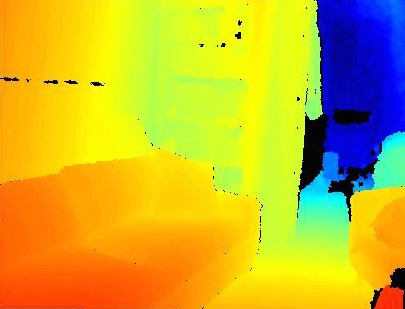
\includegraphics[height=2.1cm]{ogm_ex3.jpeg}\hspace*{0.1cm}
\hspace*{0.5cm}
    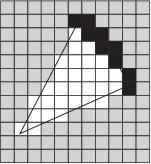
\includegraphics[height=2.1cm]{ogm_ex1.jpg}\hspace*{0.1cm}
\hspace*{0.5cm}
    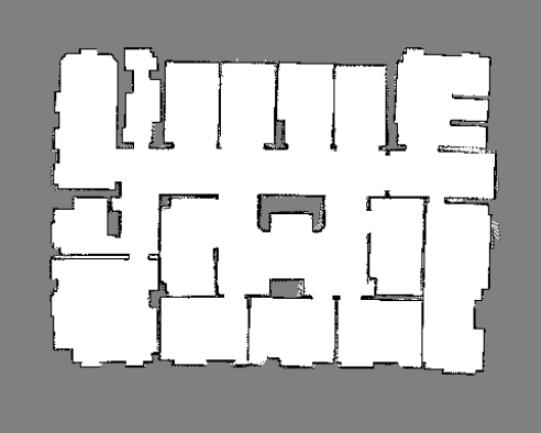
\includegraphics[height=2.1cm]{ogm_ex2.png}\hspace*{0.1cm}
}
\end{figure}}

\end{frame}






\begin{frame}
\frametitle{Problem Definition}
%\framesubtitle{Problem Definition}

\begin{itemize}
	\item The Map and the Robot
	\begin{itemize}
	\item Map $m$ is composed of $n_m$ grid cells with known location and size
	\item The $i$-th grid cell $\mathbf{m}_i$ is a \emph{static binary} random variable, independent of other grid cells: $P(m)=P(\mathbf{m}_1,\mathbf{m}_2,\ldots,\mathbf{m}_{n_m})=\prod_{i=1}^{n_m}P(\mathbf{m}_i)$
	\item \emph{Pose} $X_t$ is known, containing robot \emph{position} and \emph{attitude}
	\end{itemize}
\vspace*{0.0cm}\pause
\end{itemize}
\begin{minipage}[t]{7.0cm}
\begin{itemize}
	\item Depth Measurements
	\begin{itemize}
	\item Each measurement origin and direction is known \emph{deterministically}
	\item A measurement \emph{scan} $Z_t=\braces{z_{t,1},z_{t,2},\ldots,z_{t,n_z}}$ contains $n_z$ measurement \emph{rays} (depths)% at the $t$-th time step, and the history of measurement scans $Z_{1:t}$ is known
\item The \emph{forward sensor model} is known from the sensor properties
\end{itemize}
\end{itemize}
\end{minipage}
\begin{minipage}[t]{3.0cm}
%The \emph{forward sensor model} is the probability density distribution $p(z_{t,l}|m,X_{t})$  known from the sensor properties
\hspace*{0.25cm}
\begin{figure}[!htbp]
\vspace*{-0.25cm}
%\vspace*{0.25cm}
\centerline{
    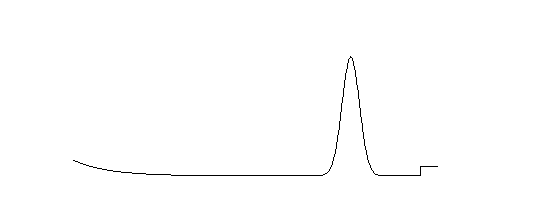
\includegraphics[width=3.5cm]{BeamModel.png}\hspace*{0.1cm}
    }
\vspace*{0.25cm}
\centerline{
    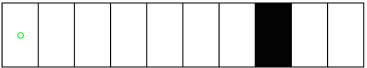
\includegraphics[width=2.5cm]{1D_True_Grid.png}\hspace*{0.1cm}
%    \hspace*{0.75cm}
    }
{Beam Model for Range Finders}
\end{figure}

\end{minipage}



\end{frame}

\begin{frame}
\frametitle{Problem Definition}

\begin{itemize}
	\item Bayesian Framework
	\begin{itemize}
	\item Markov Assumption: latest a priori cell occupancy probabilities capture the information from all prior observations
	\item Log-Odds Ratio: popular representation due to simple additive update structure and probability truncation avoidance, but requires the \emph{assumption}
	\begin{align*}
		P(Z_t|\mathbf{m}_i,X_{1:t},Z_{1:t-1})\approx P(Z_t|\mathbf{m}_i,X_t)
	\end{align*}
	\end{itemize}
\vspace*{0.0cm}\pause
	\item Inverse Sensor Model
	\begin{align*}
&P(\mathbf{m}_i|z_{t,l},X_{1:t},Z_{1:t-1})\nonumber
\\
&=\eta_{t,l}\sum_{m\in\mathcal{M}_i}p(z_{t,l}|m,X_{t})P(m|X_{1:t-1},Z_{1:t-1}).
\end{align*}
	\begin{itemize}
	\item Given $n$ grid cells: $\mathcal O(2^n)$ is \emph{computationally intractable}, motivating a different solution
	\end{itemize}
\end{itemize}

\end{frame}

\begin{frame}
\frametitle{Inexact Solutions}

\begin{minipage}[t]{7.0cm}
\begin{itemize}
	\item Approximate a function for the inverse sensor model based on intuition
	\begin{itemize}
		\item Simple to implement, but mathematically inaccurate
	\end{itemize}
\end{itemize}
\end{minipage}
\begin{minipage}[t]{3.0cm}
\begin{figure}[!htbp]
\centerline{
    \vspace*{-0.5cm}
%	\hspace*{0.25cm}
    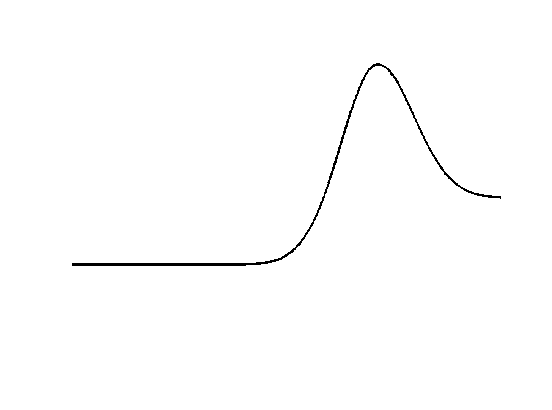
\includegraphics[width=4.0cm]{Approx_ISM_shortened.png}\hspace*{0.1cm}
    }
\centerline{
    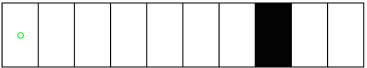
\includegraphics[width=3.5cm]{1D_True_Grid.png}
%    \hspace*{0.75cm}
    }
		\end{figure}
\end{minipage}
\vspace*{-0.5cm}
\vspace*{0.0cm}\pause
\begin{itemize}
	\item Find a solution through learning
	\begin{itemize}
		\item Simulate maps, poses, and measurements and use learning to obtain an inverse sensor model
		\item Complicated, unclear how these parameters are chosen
	\end{itemize}
	\vspace*{0.0cm}\pause
	\item Goal: design a \emph{simple} and \emph{accurate} occupancy grid mapping method avoiding log-odds ratio assumptions
\end{itemize}


\end{frame}





\begin{frame}
\frametitle{New Approach: Grouping}

\begin{itemize}
    \item Main idea: make use of occupancy grid mapping \emph{assumptions} and extract \emph{patterns} from probabilistic properties to find a \emph{computationally-efficient} solution
	\begin{itemize}
		\item Since the origin and direction of each measurement ray is known deterministically, the set of grid cells that the ray intersects is \emph{known through geometry}
		\item A depth reading follows the forward sensor model, which \emph{only depends} on the first occupied grid cell along the measurement ray
	\end{itemize}
\end{itemize}
\setcounter{subfigure}{0}
% uncomment
\begin{figure}
  \centering
  \begin{subfigure}[t]{.45\linewidth}
    \centering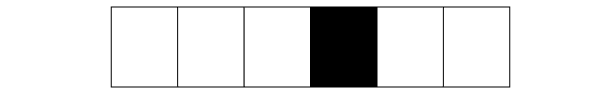
\includegraphics[width=\linewidth]{rkplus_1.png}
  \end{subfigure}
  \begin{subfigure}[t]{.45\linewidth}
    \centering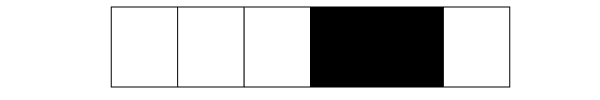
\includegraphics[width=\linewidth]{rkplus_2.png}
  \end{subfigure}
    \begin{subfigure}[t]{.45\linewidth}
    \centering
\includegraphics[width=\linewidth]{rkplus_3.png}
  \end{subfigure}
  \begin{subfigure}[t]{.45\linewidth}
    \centering
\includegraphics[width=\linewidth]{rkplus_4.png}
  \end{subfigure}
\end{figure}

\end{frame}




\begin{frame}
\frametitle{Bayesian Update}

\begin{itemize}
	\item Unnormalized Probability:
	\begin{align*}
\tilde P(\mathbf{r}_{k}|z,X_{1:t},Z_{1:t-1})
&=\mathbf{P}_k^-
\bigg[\sum_{i=1}^{k-1}\bigg\{\prod_{j=0}^{i-1}\bar{\mathbf{P}}_j^-\bigg\}p(z|\mathbf{r}_{i+},X_t)\mathbf{P}_k^-\bigg]\nonumber\\
&\qquad + \bigg\{\prod_{j=0}^{k-1}\bar{\mathbf{P}}_j^-\bigg\}p(z|\mathbf{r}_{k+},X_t)\mathbf{P}_k^-
\end{align*}
	\item Normalizer:
	\begin{align*}
\label{eqn:allEta}
\eta
&=
\bigg[\sum_{i=1}^{n_{r}+1}\bigg\{\prod_{j=0}^{i-1}\bar{\mathbf{P}}_j^-\bigg\} p(z|\mathbf{r}_{i+},X_t)\mathbf{P}_k^-\bigg]^{-1}
\end{align*}
	\item Solution: $P(\mathbf{r}_{k}|z,X_{1:t},Z_{1:t-1})=\eta\tilde P(\mathbf{r}_{k}|z,X_{1:t},Z_{1:t-1})$
	\item \emph{Linear Complexity} ($\mathcal{O}(n)$ for \emph{all} $n$ cells in FOV)
\end{itemize}
\end{frame}

% Ray Casting

\begin{frame}
\frametitle{Ray Casting}

\begin{itemize}
	\item Required for 2D and 3D occupancy grid maps
	\item Main idea: use simple geometry to find the distance from the robot sensor to each cell intersected by the measurement ray
\end{itemize}

\begin{figure}[!ht]
    \centering
    \begin{subfigure}[t]{0.4\columnwidth}
        \centering
        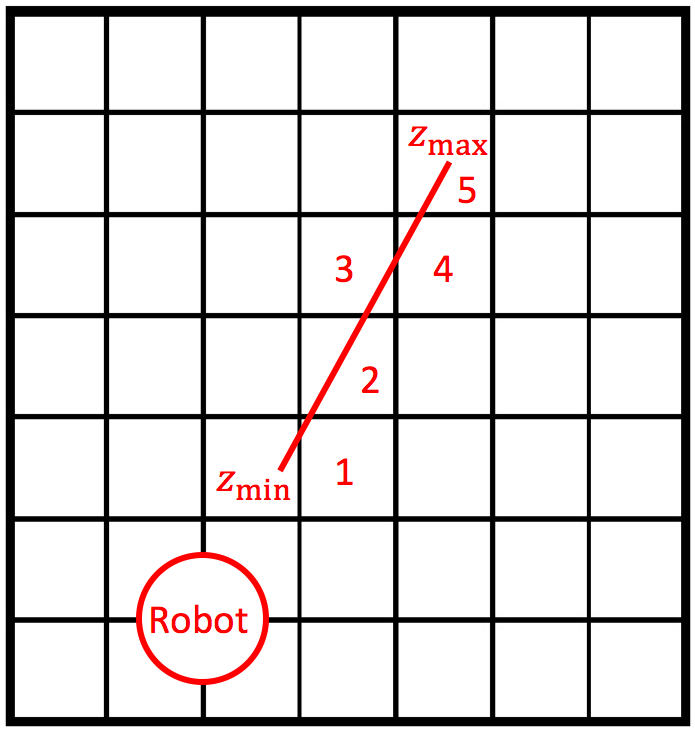
\includegraphics[width=\textwidth]{RayCastingIllustration.png}
%        \label{fig:penn_map_total}
    \end{subfigure}
    \hspace*{0.05\columnwidth}
    \begin{subfigure}[t]{0.4\columnwidth}
        \centering
        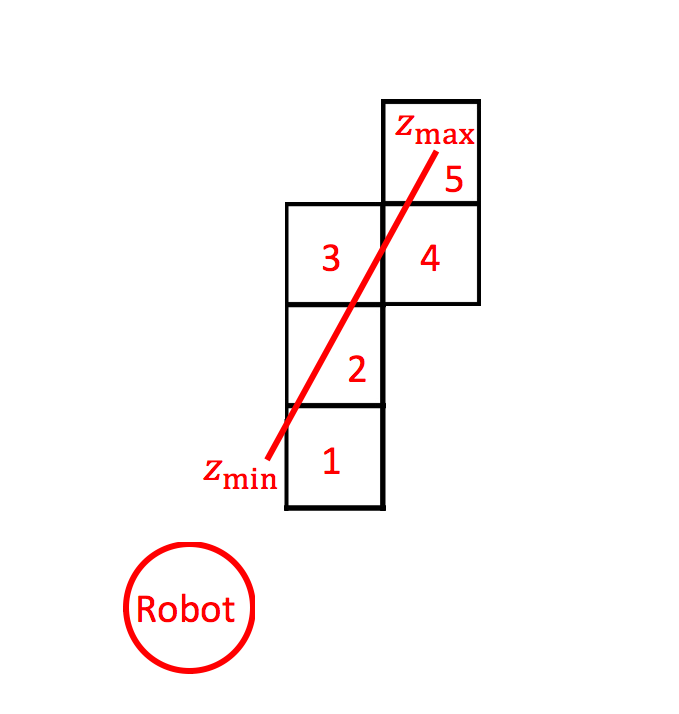
\includegraphics[width=\textwidth]{RayCastIllustrationReducedMapOnly.png}
%        \label{fig:penn_map_zoom}
    \end{subfigure}
\end{figure}

\end{frame}

\begin{frame}
\frametitle{Full Measurement Scan}

\begin{itemize}
	\item Two Methods
	\begin{itemize}
		\item \emph{Ray-By-Ray Inverse Sensor Model}: each measurement ray is evaluated individually for updating the map
		\item \emph{Synergistic Scan Inverse Sensor Model}: all measurement rays are evaluated simultaneously
	\end{itemize}
\end{itemize}

\end{frame}


\begin{frame}
\frametitle{Ray-By-Ray Inverse Sensor Model}

\begin{itemize}
	\item Main idea: given a scan of measurement rays, update the map based on each measurement ray \emph{individually} and \emph{sequentially}
	\item Conditional probability:
	\begin{align*}
		P(\mathbf{m}_i|X_{1:t}&,Z_{1:t})\nonumber\\&
		=P((\dots(((\mathbf{m}_i|X_{1:t},Z_{1:t-1})|z_{t,1})|z_{t,2})|\ldots)|z_{t,n_z})
	\end{align*}
	\item Benefit: the measurement rays maintain some dependency as they capture the same map
	\item Drawback: the best order for evaluating rays is not necessarily chosen
\end{itemize}

\end{frame}

\begin{frame}
\frametitle{Synergistic Scan Inverse Sensor Model}

\begin{itemize}
	\item Main idea: consider every measurement ray inside a scan \emph{simultaneously} to update all grid cells inside the FOV
	\item Probability derived from a Bayesian approach:
	\begin{align*}
		P(\mathbf{m}_i|X_{1:t},Z_{1:t})
		&=\xi_i P(\mathbf{m}_i|{X_{1:t-1}},Z_{1:t-1})\nonumber\\&\quad\times
		\prod_{l\in\mathcal L_i}
		\hat P(\mathbf{r}_{l,k}|z_{t,l},X_{1:t},Z_{1:t-1}),
		\\
		\hat P(\mathbf{r}_{l,k}|z_{t,l},X_{1:t},Z_{1:t-1})&
		\triangleq \frac{\tilde P(\mathbf{r}_{l,k}|z_{t,l},X_{1:t},Z_{1:t-1})}{P(\mathbf{m}_i|X_{1:t-1},Z_{1:t-1})}
	\end{align*}
	\item Benefit: synergistic update provides a method where all rays are considered simultaneously
	\item Drawback: required assumption that the measurement rays are independent, though they capture the same map
\end{itemize}

\end{frame}



\begin{frame}
\frametitle{Numerical Example}

\begin{minipage}[t]{5.0cm}
\vspace*{0.5cm}
\begin{itemize}
	\item A standard \emph{approximate} inverse sensor model technique is compared with the proposed \emph{exact} method
\end{itemize}
\end{minipage}
\begin{minipage}[t]{5.0cm}
%\vspace*{0.5cm}
\begin{figure}[!htbp]
    \centering
    \begin{subfigure}{0.5\textwidth}
        \centering
        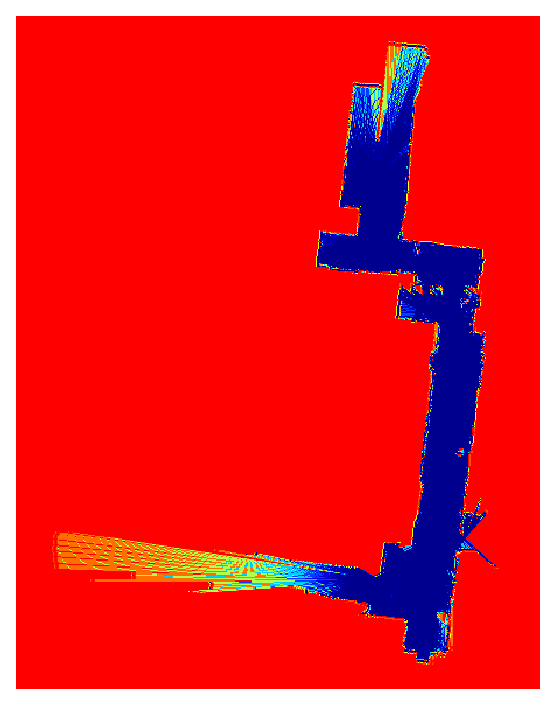
\includegraphics[width=\textwidth]{AISM_Image_inf_19.pdf}
        \caption*{Approximate}
    \end{subfigure}
    \hspace*{-0.1\textwidth}
    \begin{subfigure}{0.5\textwidth}
        \centering
        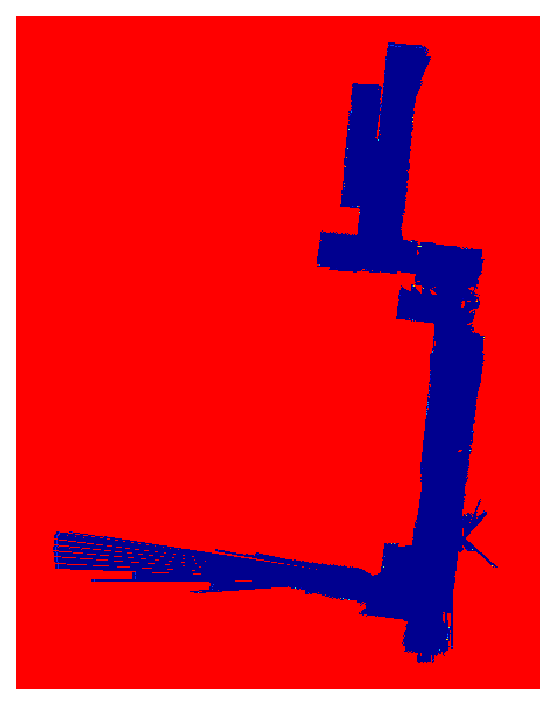
\includegraphics[width=\textwidth]{EISM_Image_inf_19.pdf}
        \caption*{Exact}
    \end{subfigure}
\end{figure}
\end{minipage}


\begin{itemize}
\item The exact algorithm yields a more \emph{certain} map from the same measurement set
\end{itemize}

\end{frame}

\begin{frame}
\frametitle{Probabilistic Occupancy Grid Mapping Conclusions}

\begin{itemize}
	\item The proposed novel Bayesian solution to the inverse sensor model provides the exact solution without approximate functions or learned solutions
	\item The computational complexity is linear with respect to the number of cells considered, making real-time implementation possible
	\item 2D and 3D maps are updated with ray casting and ray-by-ray combination
\end{itemize}

\end{frame}

\section*{}
\subsection*{Entropy-Based Autonomous Exploration}

\begin{frame}
\frametitle{Autonomous Exploration}

\begin{itemize}
	\item Goal: determine robotic actions that maximize map information
	\item Solution: predict future map uncertainty and travel distance to select an optimal pose
\end{itemize}

\end{frame}




\begin{frame}
\frametitle{Existing Exploration Approaches}

\begin{itemize}
	\item Frontier-Based Exploration
	\begin{itemize}
		\item A robot identifies boundaries of free and uncertain cells
		\item The robot moves toward these frontiers, thereby pushing back the boundaries
		\item Heuristic, suboptimal
	\end{itemize}
	\vspace*{0.0cm}\pause
	\item Entropy-Based Approaches
	\begin{itemize}
		\item Probabilities from the occupancy grid map are approximate
		\item Usage of ``hallucination measurements'': assume that $\text{E}[H(P(\mathbf{m}_i|z))]\approx H(P(\mathbf{m}_i|\text{E}[z]))$
	\end{itemize}
	\vspace*{0.0cm}\pause
	\item Proposed Approach
	\begin{itemize}
		\item Use occupancy grid map probabilities
		\item Solve $\text{E}[H(P)]$ and select future poses to maximize map information
	\end{itemize}
\end{itemize}
\end{frame}

\begin{frame}
\frametitle{Entropy Definition}
\begin{itemize}
        	\item Uncertainty-Based Exploration
	\begin{itemize}
		\item Main idea: choose robot motions that minimize the uncertainty of the occupancy grid map
		\item Equivalently maximize map information gain
	\end{itemize}
\end{itemize}
\begin{minipage}[t]{7.0cm}
\begin{itemize}
	\item Entropy
	\begin{itemize}		
		\item \emph{Shannon's entropy} serves as an uncertainty measure
		\begin{align*}
			H(P)=-P\log P-\bar{P}\log \bar{P}%-(1-P)\log(1-P)
		\end{align*}
		with cell occupancy probability $P$ and complement $\bar{P}=1-P$
		\item Entropy $H$ is maximized when $P=0.5$ and minimized as $P\rightarrow0$ or $P\rightarrow1$
	\end{itemize}
\end{itemize}
\end{minipage}
\begin{minipage}[t]{3.0cm}
\vspace*{0.5cm}
\begin{figure}[!htbp]
	\centerline{
		\hspace*{1.25cm}
   		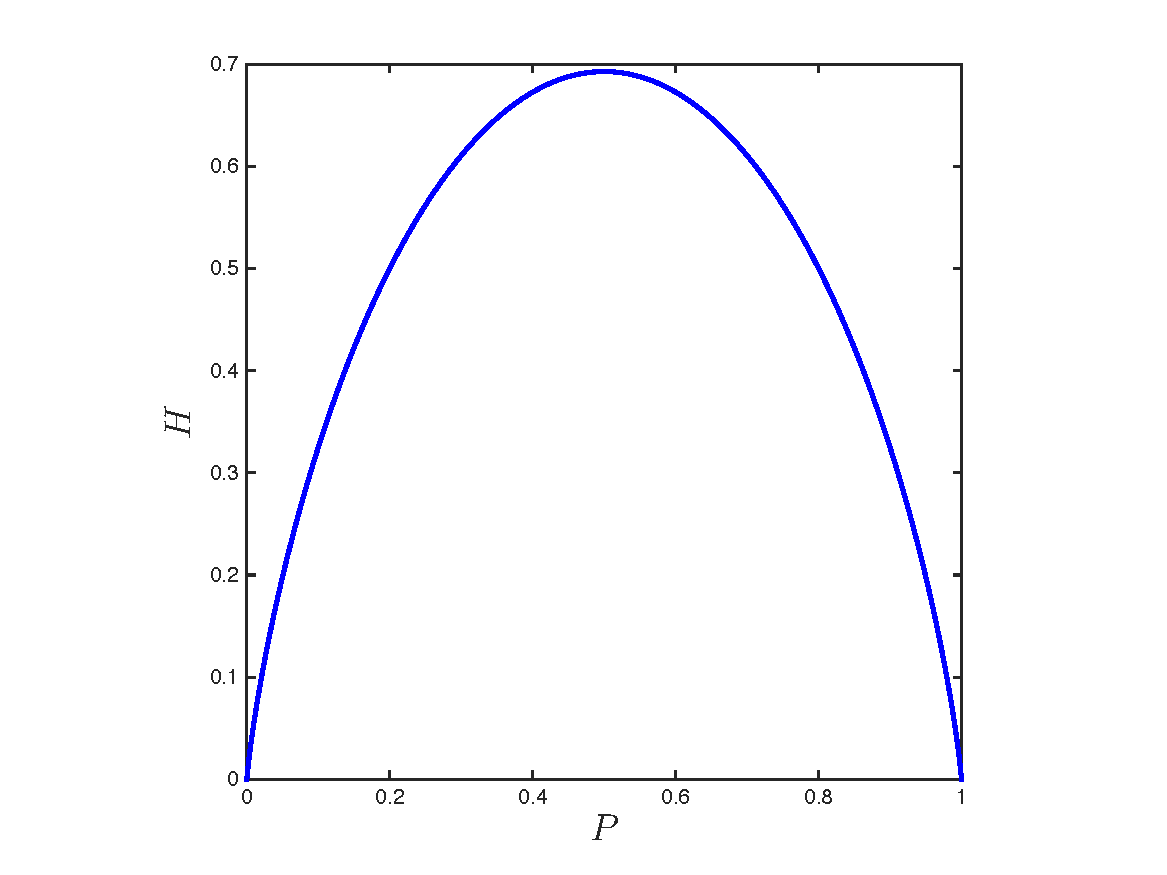
\includegraphics[width=5.0cm]{H_Plotted_square.pdf}%\hspace*{0.1cm}
	}
\end{figure}
\end{minipage}

\end{frame}



\begin{frame}
\frametitle{Expected Information Gain}

\begin{itemize}
	\item Main Idea: determine the benefit of future poses based on how their measurements are expected to improve the map
	\vspace*{0.0cm}\pause
	\item Goal: decrease total map entropy:
	\begin{align*}
		H(P(m))&=\sum_{i=1}^{n_m}H(P(\mathbf{m}_i))
	\end{align*}
	\vspace*{0.0cm}\pause
	\item Measurement Ray Expected Information Gain:
	\begin{align*}
		\text{E}[H(P(m|x_c,z_{c}))]&=\sum_{k=1}^{n_{r}+1}\bigg\{H(P(m|x_c,z_{c,k}))P(z_{c,k}|x_c)\bigg\}
		\\
		P(z_{c,k}|x_c)&=\frac{p(z_{c,k}|x_c)}{\sum_{i=1}^{n_{r}+1}p(z_{c,i}|x_c)}=\frac{\eta_{c,k}^{-1}}{\sum_{i=1}^{n_{r}+1}\eta_{c,i}^{-1}}
		\\
		\mathcal I(x_c,z_{c})&=H(P(m))-\text{E}[H(P(m|x_c,z_{c}))]
	\end{align*}
\end{itemize}

\end{frame}




\begin{frame}
\frametitle{Expected Information Gain Computation}

\begin{itemize}
	\item \emph{Squared Complexity}: $\mathcal O(n_r^2)$ for $n_r$ cells along the ray
	\vspace*{0.0cm}\pause
	\item Two Approaches:
	\begin{itemize}
		\vspace*{0.0cm}\pause
		\item Decrease the cells considered by selecting $n_p$ most probable cells: $\mathcal O(n_r^2)$ reduces to $\mathcal O(n_p^2)$
		\vspace*{0.0cm}\pause
		\item Use 3D cells in a 2D \emph{projection}
\begin{figure}
  \centering
  \begin{subfigure}[t]{.3\linewidth}
    \centering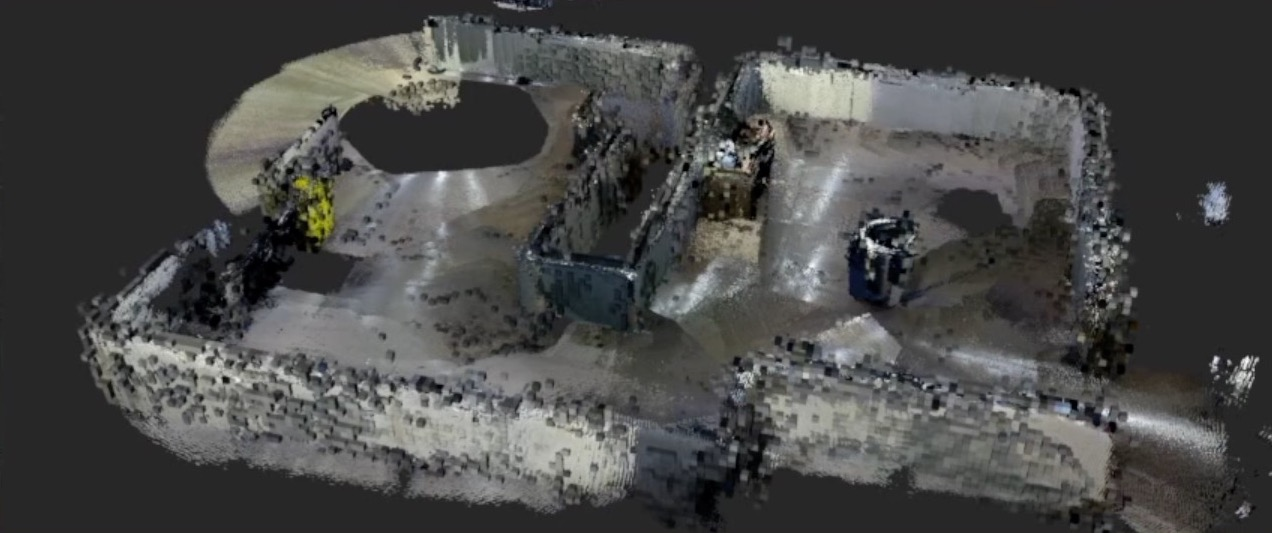
\includegraphics[height=.75\linewidth]{experiment_ogm3D_2min47sec.jpg}
    \caption*{\ \ \ \ \ \ \ \ \ \ \ \ \ \ 3D Map}
  \end{subfigure}
  \hspace*{0.25\linewidth}
  \begin{subfigure}[t]{.3\linewidth}
    \centering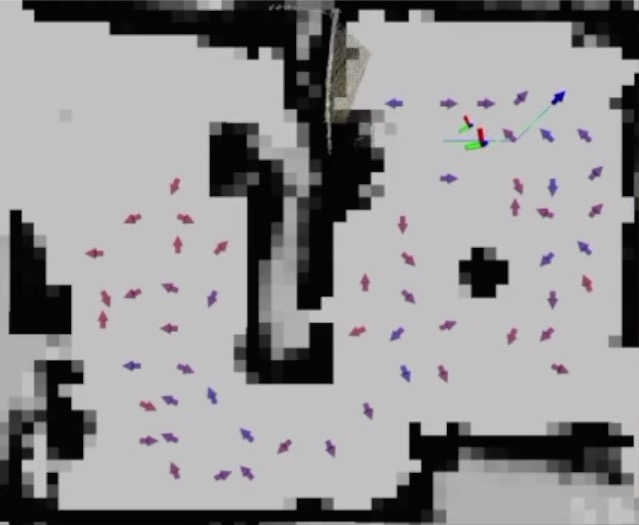
\includegraphics[height=.75\linewidth]{experiment_2min47sec.jpg}
    \caption*{2D Projection}
  \end{subfigure}
\end{figure}
	\end{itemize}
\end{itemize}

\end{frame}

\begin{frame}
\frametitle{Pose Selection}

\begin{itemize}
	\item Main Idea: select the future pose that maximizes map information gain while accounting for travel distance
	\vspace*{0.0cm}\pause
	\item Attitude Selection: choose the attitude that covers the candidate measurement rays with largest objective function summation
\begin{figure}
\centerline{
	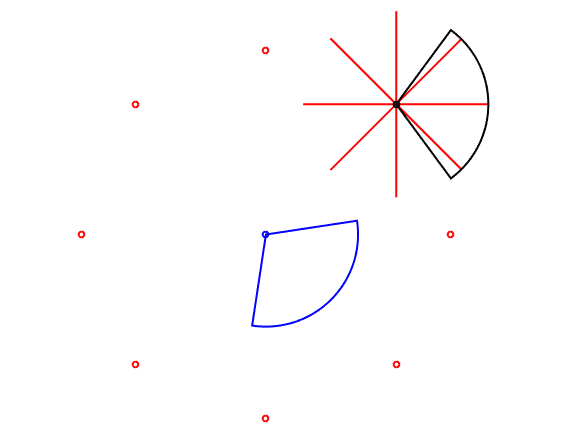
\includegraphics[height=0.35\linewidth]{ExampleOptimalPose.png}
%\begin{picture}(0,0)(0,0)
%\setlength{\unitlength}{0.1\linewidth}\scriptsize
%\put(4.4,2.1){\color{blue}$X_t$}
%\put(5.9,1.9){\color{red}$x_1$}
%\put(2.9,2.0){\color{red}$x_5$}
%\put(4.4,3.6){\color{red}$x_3$}
%\put(4.4,0.6){\color{red}$x_7$}
%\put(5.4,3.0){\color{red}$x_2$}
%\put(3.3,3.1){\color{red}$x_4$}
%\put(3.3,1.0){\color{red}$x_6$}
%\put(5.4,1.0){\color{red}$x_8$}
%\put(6.8,3.1){\color{red}$z_{2,1}$}
%\put(4.5,3.1){\color{red}$z_{2,5}$}
%\put(5.6,4.1){\color{red}$z_{2,3}$}
%\put(5.6,2.2){\color{red}$z_{2,7}$}
%\put(6.5,3.7){\color{red}$z_{2,2}$}
%\put(4.9,3.8){\color{red}$z_{2,4}$}
%\put(5.0,2.5){\color{red}$z_{2,6}$}
%\put(6.5,2.5){\color{red}$z_{2,8}$}
%\put(6.1,2.9){$X_c^*$}
%\end{picture}
}
\vspace*{-0.05\linewidth}
\end{figure}
	\item The attitude $R_c$ is selected for all candidates: the expected information gain becomes $\mathcal I(X_c)$ where $X_c=\braces{x_c,R_c}$
\end{itemize}

\end{frame}

\begin{frame}
\frametitle{Pose Selection}

\begin{itemize}
	\item Travel Distance: generate a cost map from the occupancy grid to obtain distances to each candidate pose $d(x_c)$
	\vspace*{0.0cm}\pause
	\item Bump Function: use a bump function \begin{align*}f(d)=\exp\braces{-\frac{d^2}{2\sigma^2}}+\gamma, \quad \sigma>0, \quad \gamma>0\end{align*} to incentivize the robot to explore more locally until nearby spaces are well-known
	\begin{figure}
	\vspace*{-0.015\linewidth}
\centering
	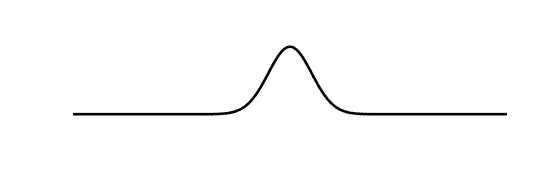
\includegraphics[width=0.8\linewidth]{GaussianBumpFunFlat.png}
		\vspace*{-0.015\linewidth}
\end{figure}
	% C++: exp(-0.5*distAway*distAway/sigSqrd)+minFunVal GaussianBumpFunFlat.png
	\vspace*{0.0cm}\pause
	\item Select the pose that maximizes the product \begin{align*}X^*=\argmax_{X_c}{\mathcal I(X_c)f(d(x_c))}\end{align*}
\end{itemize}

\end{frame}


\begin{frame}
\frametitle{Collision-Free Path}

\begin{itemize}
	\item Using the cost map from before, \emph{Dijkstra's algorithm} is completed by finding the waypoints from the desired candidate back to the current location
	\vspace*{0.0cm}\pause
	\item These waypoints serve as input to a \emph{constrained polynomial least squares trajectory}
	\begin{itemize}
		\item Each trajectory is solved independently as a function of time, i.e. $x(t)$, $y(t)$
		\item Starting and terminal locations are fixed
		\item Segments patched together have the same position and velocity at the connection
	\end{itemize}
	\vspace*{0.0cm}\pause
	\item A \emph{geometric controller} tracks the trajectory without \emph{singularities} or \emph{ambiguities}
	\vspace*{0.0cm}\pause
	\item The mapping, exploration, and control run in \emph{real-time}
\end{itemize}

\end{frame}

% TODO: uncomment!
%\begin{frame}
%	\frametitle{Numerical Results}
%	\centering{
%		\includemedia[
%  		width=0.720\textwidth,
%  		height=0.576\textwidth,
%  		activate=pageopen,
%  		addresource=IRL.mp4,
%  		flashvars={source=IRL.mp4}
%		]{}{VPlayer.swf}
%		}
%\end{frame}


%\frametitle{Experimental Results}
%	\centering{
%	\includemovie[poster,autoplay]{0.720\textwidth}{0.576\textwidth}{JIRS16_experiment_SideBySide_speedup8x.mov}}
%\end{frame}


\begin{frame}
\frametitle{Autonomous Exploration Conclusions}

\begin{itemize}
	\item Other approaches use heuristic frontiers or entropy of expected measurements
	\item The proposed approach solves for the expected value of future map entropy directly
	\item Several sample future measurement rays and Dijkstra's cost map combine in an objective function for optimality
	\item Numerical simulations show a large 2D environment, and this approach can be extended to 3D environments
\end{itemize}

\end{frame}

\section*{}
\subsection*{Multi-Vehicle Coordination}

\begin{frame}
\frametitle{Motivation and Goal}

\begin{itemize}
	\item Multiple agents can accomplish tasks faster and more reliably than a single agent
	\item Large groups are capable of coverage in large environments
	\item Problem: multi-vehicle map information gain optimality can be computationally intractable
	\item Solution: bidding-based solution simplifies a complicated optimization into a series of simplified optimizations
\end{itemize}

\end{frame}

\begin{frame}
\frametitle{Related Work}

\begin{itemize}
	\item Most existing bidding-based techniques deal with auctioning tasks among a few agents locally in decentralized frameworks
	\item The other approach is for a central executive to run a series of auctions
	\item Bids are discounted between auctions to coordinate the efforts based on coverage overlap
	\item Heuristic, ad hoc
\end{itemize}

\end{frame}

\begin{frame}
\frametitle{Proposed Approach}

\begin{itemize}
\item Central executive completes $n$ auctions for $n$ robots
\begin{enumerate}
	\item Each robot determines its optimal future pose, and bids the objective function
	\item The winner is awarded this future pose, and the remaining robots update their bids according to
	\begin{itemize}
		\item New expected map changes from the winner
		\item Collision-avoidance with the winner
	\end{itemize}
	\item Repeat these steps with the remaining robots
\end{enumerate}
\item The efforts are coordinated by updating bids between auctions
\end{itemize}
\end{frame}

% TODO: uncomment!
%\begin{frame}
%\frametitle{Numerical Example: SEH Second Floor}
%
%
%	\centering{
%		\includemedia[
%  		width=0.720\textwidth,
%  		height=0.576\textwidth,
%  		activate=pageopen,
%  		addresource=Multi-Vehicle Mapping and Exploration.mp4,
%  		flashvars={source=Multi-Vehicle Mapping and Exploration.mp4}
%		]{}{VPlayer.swf}
%		}
%
%
%\end{frame}


\section*{}
\subsection*{Experiments}


%
%\section*{}
%
%\begin{frame}
%\frametitle{}
%%\center
%\center{\bf \color{blue} Single-Robot Autonomous Exploration}
%\end{frame}
%
%
%\subsection*{Single-Robot Autonomous Exploration}
%
%\begin{frame}
%\frametitle{Introduction}
%\begin{itemize}
%        	\item The environment is initially uncertain, so the robot path is initially unknown
%	\item Simultaneous localization and mapping assumes robotic actions are provided
%	\item Human interaction is common to guide the robot
%	\item Goal: develop effective policies to govern robotic motion 
%\end{itemize}
%
%\end{frame}
%
%
%\begin{frame}
%\frametitle{Problem Definition}
%\begin{itemize}
%        	\item Uncertainty-Based Exploration
%	\begin{itemize}
%		\item Main idea: choose robot motions that minimize the uncertainty of the occupancy grid map
%		\item Equivalently maximize map information gain
%	\end{itemize}
%\end{itemize}
%\begin{minipage}[t]{7.0cm}
%\begin{itemize}
%	\item Entropy
%	\begin{itemize}		
%		\item \emph{Shannon's entropy} serves as an uncertainty measure
%		\begin{align*}
%			H(P)=-P\log P-\bar{P}\log \bar{P}%-(1-P)\log(1-P)
%		\end{align*}
%		with cell occupancy probability $P$ and complement $\bar{P}=1-P$
%		\item Entropy $H$ is maximized when $P=0.5$ and minimized as $P\rightarrow0$ or $P\rightarrow1$
%	\end{itemize}
%\end{itemize}
%\end{minipage}
%\begin{minipage}[t]{3.0cm}
%\vspace*{0.5cm}
%\begin{figure}[!htbp]
%	\centerline{
%		\hspace*{1.25cm}
%   		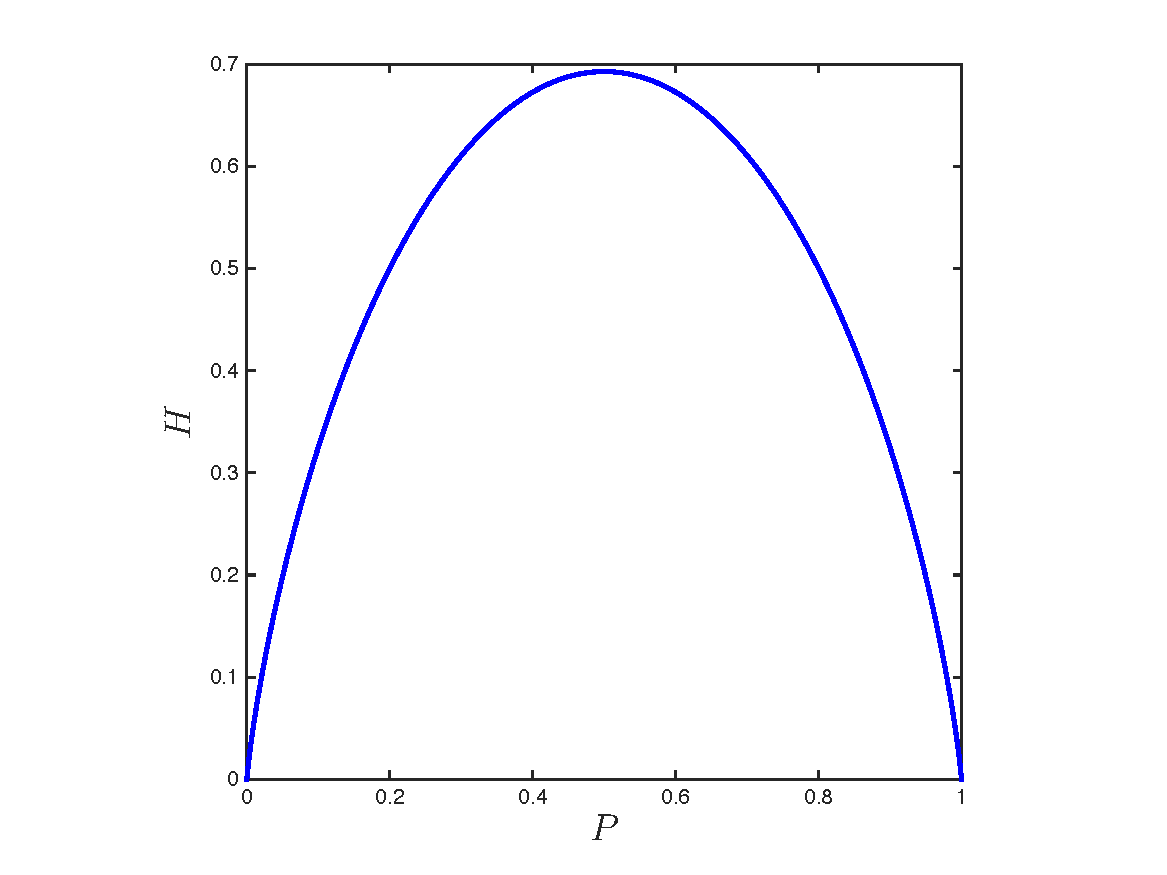
\includegraphics[width=5.0cm]{H_Plotted_square.pdf}%\hspace*{0.1cm}
%	}
%\end{figure}
%\end{minipage}
%
%\end{frame}
%
%
%
%\begin{frame}
%\frametitle{Problem Definition}
%\begin{itemize}
%        	\item Map Information Gain Maximization
%	\begin{itemize}
%		\item Goal: choose a set of optimal future poses to maximize map information gain
%		\pause
%		\item Challenge: the complete set cannot be calculated accurately with an initially highly-uncertain environment
%		\pause
%		\item Solution: choose short-term optimal pose goals, reevaluating an updated map for the subsequent optimizations
%		\pause
%		\item The information gain considering candidate future pose $X_c$:% is
%		\begin{align*}
%			\mathcal I(X_c)&=H(P(m|X_{1:t},Z_{1:t}))-\text{E}\left[H(P(m|X_{1:t},Z_{1:t},X_c,Z_c))\right]
%		\end{align*}
%		\pause
%		\item Optimal pose $X^*_c$ satisfies
%		\begin{align*}
%			X_c^*=\argmax_{X_c}{\mathcal I(X_c)}
%		\end{align*}
%	\end{itemize}
%\end{itemize}
%
%
%\end{frame}
%
%
%
%\begin{frame}
%\frametitle{Related Work}
%\begin{itemize}
%        	\item Frontier-Based Exploration
%	\begin{itemize}
%		\item Main idea: robot moves toward boundaries between certain and uncertain space, takes measurements, then pushes back the boundaries
%		\item Non-entropy-based exploration
%		\item Heuristic
%	\end{itemize}
%	\pause
%	\item Entropy-Based Exploration
%	\begin{itemize}
%		\item Cell occupancy probabilities are inaccurate: inverse sensor model is heuristic or learned, and frequently estimated with Rao-Blackwellized particle filters
%		\item Inaccurate probabilities imply inaccurate entropy measures
%		\item Approaches use ``hallucination measurements'' to predict how future measurements \emph{might} affect the map uncertainty,
%		\begin{align*}
%			\text{E}\left[H(P(m|X_{1:t},Z_{1:t},X_c,Z_c))\right]\approx H(P(m|X_{1:t},Z_{1:t},X_c,\text{E}\left[Z_c\right]))
%		\end{align*}
%	\end{itemize}
%\end{itemize}
%
%
%\end{frame}
%
%
%\begin{frame}
%\frametitle{Direct Entropy Calculation}
%\begin{itemize}
%        	\item Instead of relying on frontiers or making assumptions about measurements, the expected map entropy is \emph{calculated directly} by the law of total expectation:
%	\begin{align*}
%		\text{E}[H(P(m|X,z))]=\int_{z_\text{min}}^{z_\text{max}}
%		H(P(m|X,z))p(z|X)dz,
%	\end{align*}
%	\item The robot pose is chosen to maximize map information gain from this expectation
%	\item Dijkstra's algorithm provides collision-free waypoints for the robot path
%	\item Smooth trajectory: constrained polynomial least squares 
%\end{itemize}
%
%
%\end{frame}
%
%
%\begin{frame}
%\frametitle{Numerical Example}
%\begin{itemize}
%        	\item A benchmark example floor plan is explored and mapped using the proposed mapping and exploration algorithms
%	\item Simulations in Robot Operating System (ROS)
%\end{itemize}
%\begin{figure}
%    \centering
%    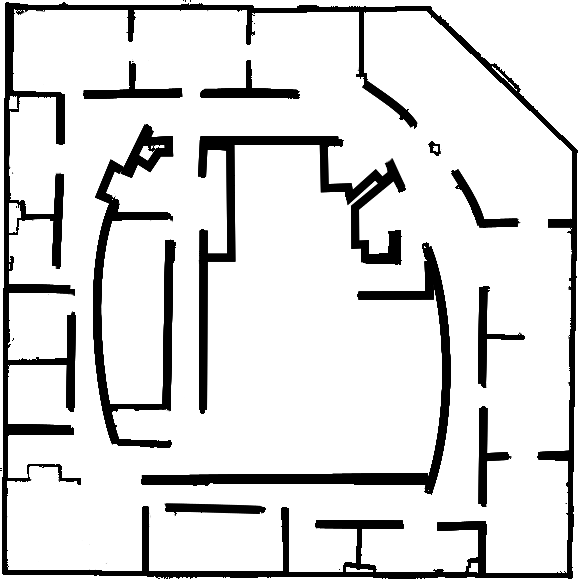
\includegraphics[width=0.4\textwidth]{intel_clean.png}
%    \caption*{Modified Intel Research Lab floor plan form the SLAM benchmark}
%\end{figure}
%
%\end{frame}
%
%%\begin{frame}
%%\frametitle{Numerical Results}
%%	\centering{
%%	\includemovie[poster,autoplay]{0.720\textwidth}{0.576\textwidth}{../../Fig/JIRS16_simulation_speedup10x_then_speedup100x.mov}}
%%\end{frame}
%
%\begin{frame}
%\frametitle{Numerical Results}
%
%\begin{figure}[!ht]
%    \centering
%    \begin{subfigure}[t]{0.2\columnwidth}
%        \centering
%        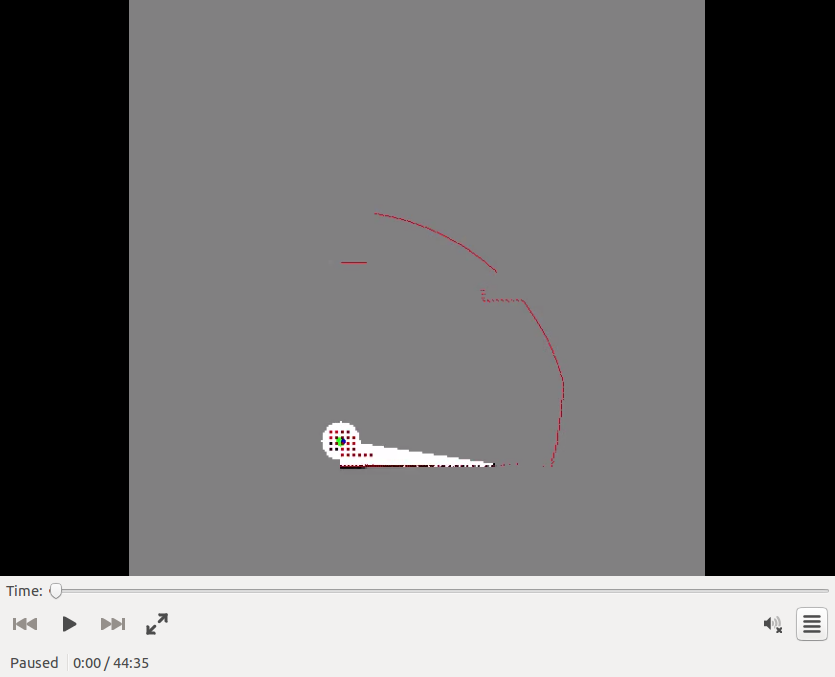
\includegraphics[trim = {4.6cm 3.8cm 4.6cm 0}, clip, width=\textwidth]{0min.png}
%        \caption*{$t=0$ min}
%        \label{fig:IRL0min}
%    \end{subfigure}
%    \begin{subfigure}[t]{0.2\columnwidth}
%        \centering
%        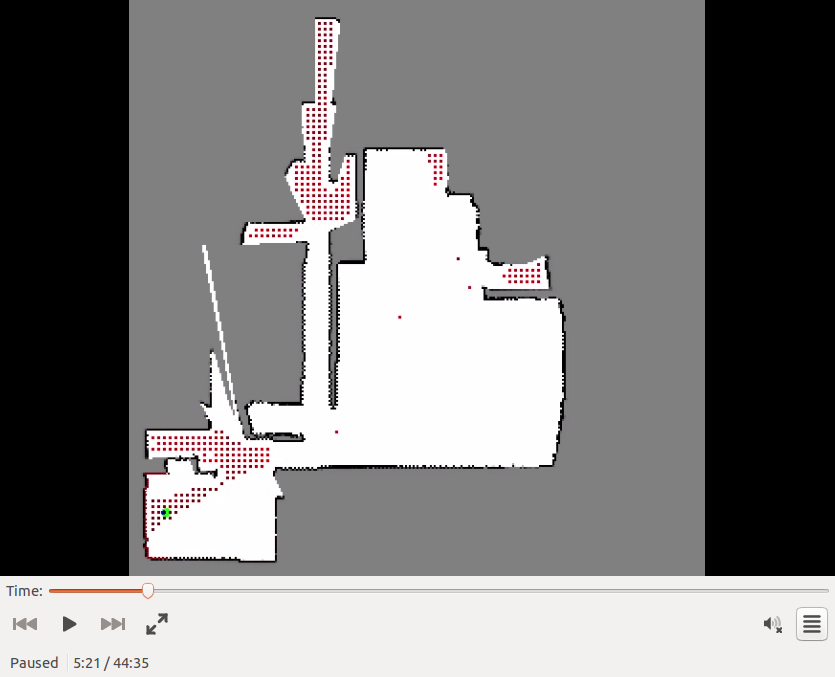
\includegraphics[trim = {4.6cm 3.8cm 4.6cm 0}, clip, width=\textwidth]{5min.png}
%        \caption*{$t=5$ min}
%        \label{fig:IRL5min}
%    \end{subfigure}
%    \begin{subfigure}[t]{0.2\columnwidth}
%           \centering
%           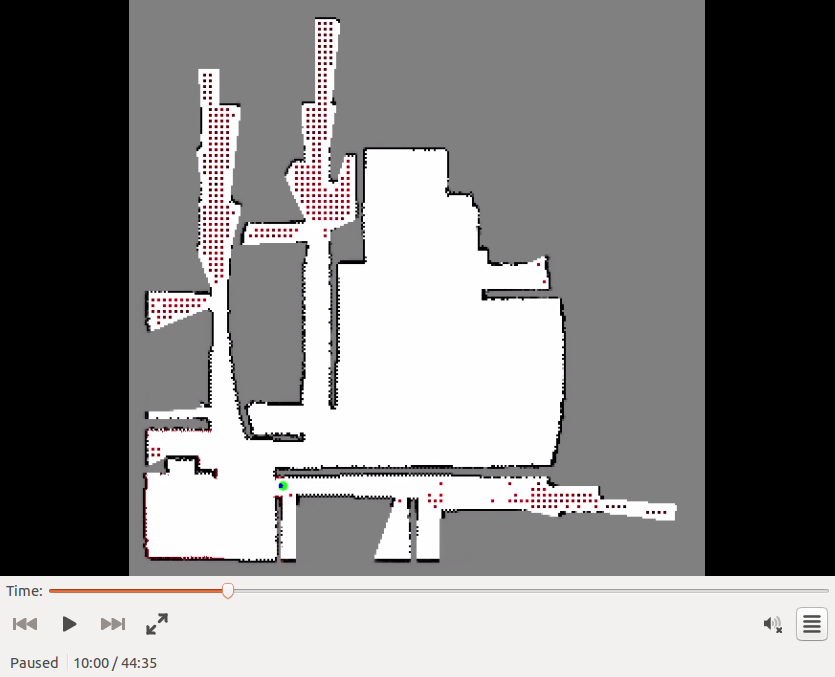
\includegraphics[trim = {4.6cm 3.8cm 4.6cm 0}, clip, width=\textwidth]{10min.png}
%        \caption*{$t=10$ min}
%        \label{fig:IRL10min}
%    \end{subfigure}
%    \begin{subfigure}[t]{0.2\columnwidth}
%           \centering
%           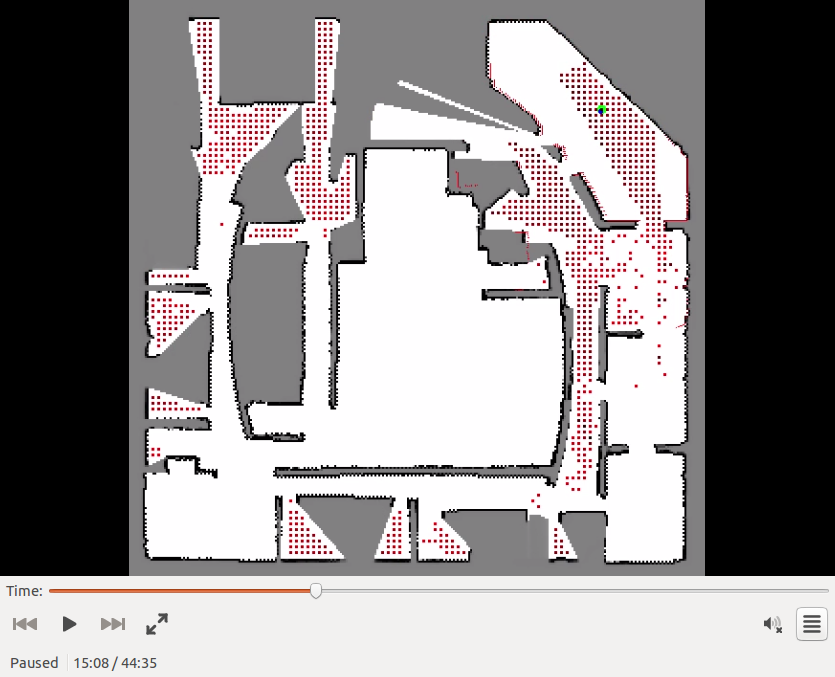
\includegraphics[trim = {4.6cm 3.8cm 4.6cm 0}, clip, width=\textwidth]{15min.png}
%        \caption*{$t=15$ min}
%        \label{fig:IRL15min}
%    \end{subfigure}
%    \begin{subfigure}[t]{0.2\columnwidth}
%         \centering
%         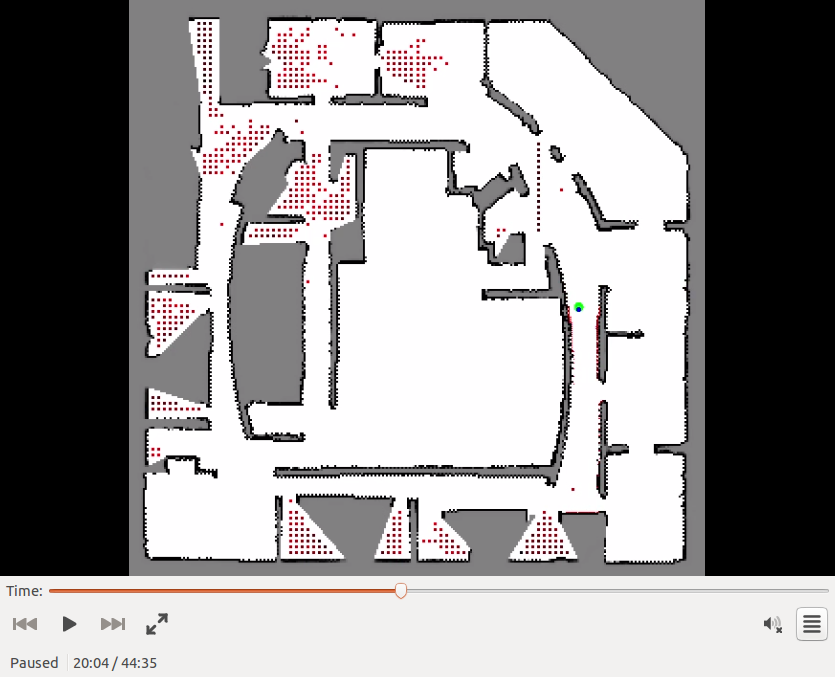
\includegraphics[trim = {4.6cm 3.8cm 4.6cm 0}, clip, width=\textwidth]{20min.png}
%        \caption*{$t=20$ min}
%        \label{fig:IRL20min}
%    \end{subfigure}
%    \begin{subfigure}[t]{0.2\columnwidth}
%           \centering
%           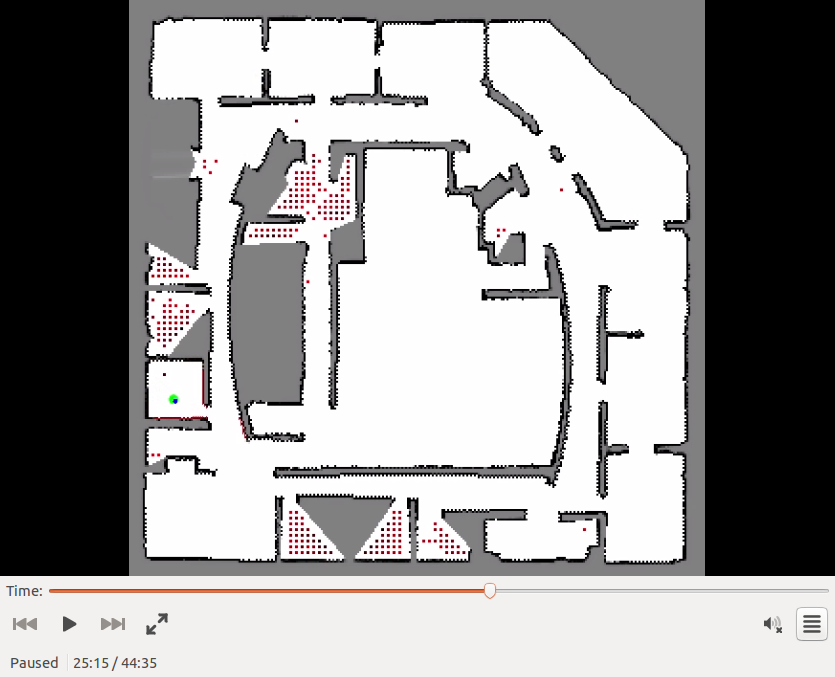
\includegraphics[trim = {4.6cm 3.8cm 4.6cm 0}, clip, width=\textwidth]{25min.png}
%        \caption*{$t=25$ min}
%        \label{fig:IRL25min}
%    \end{subfigure}
%    \begin{subfigure}[t]{0.2\columnwidth}
%           \centering
%           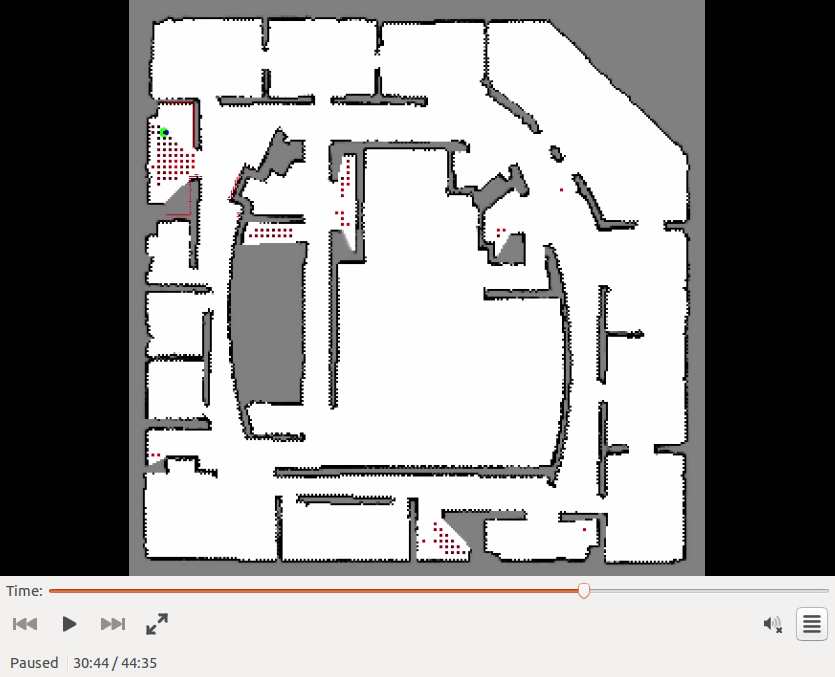
\includegraphics[trim = {4.6cm 3.8cm 4.6cm 0}, clip, width=\textwidth]{30min.png}
%        \caption*{$t=30$ min}
%        \label{fig:IRL30min}
%    \end{subfigure}
%    \begin{subfigure}[t]{0.2\columnwidth}
%           \centering
%           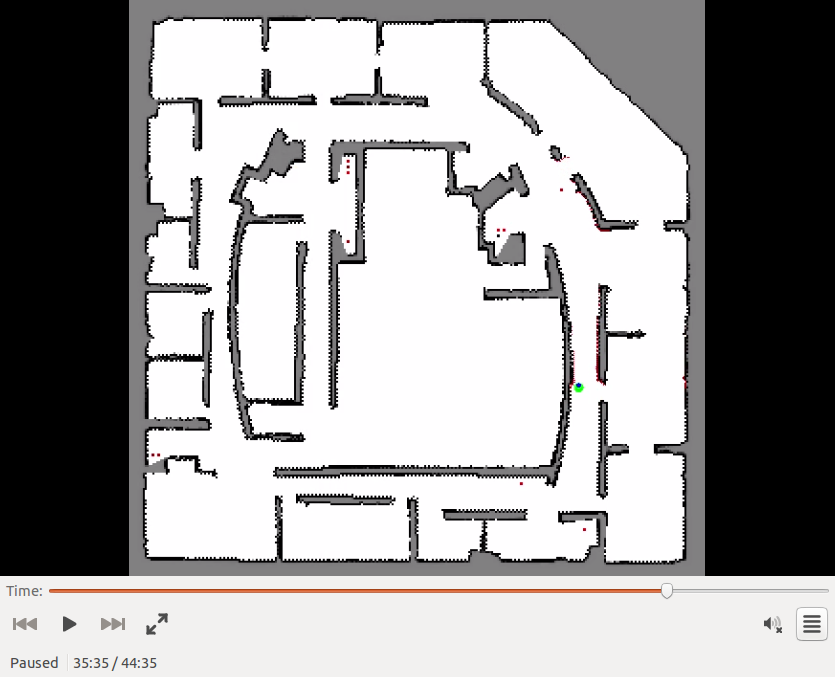
\includegraphics[trim = {4.6cm 3.8cm 4.6cm 0}, clip, width=\textwidth]{35min.png}
%        \caption*{$t=35$ min}
%        \label{fig:IRL35min}
%    \end{subfigure}
%%    \begin{subfigure}[t]{0.2\columnwidth}
%%           \centering
%%           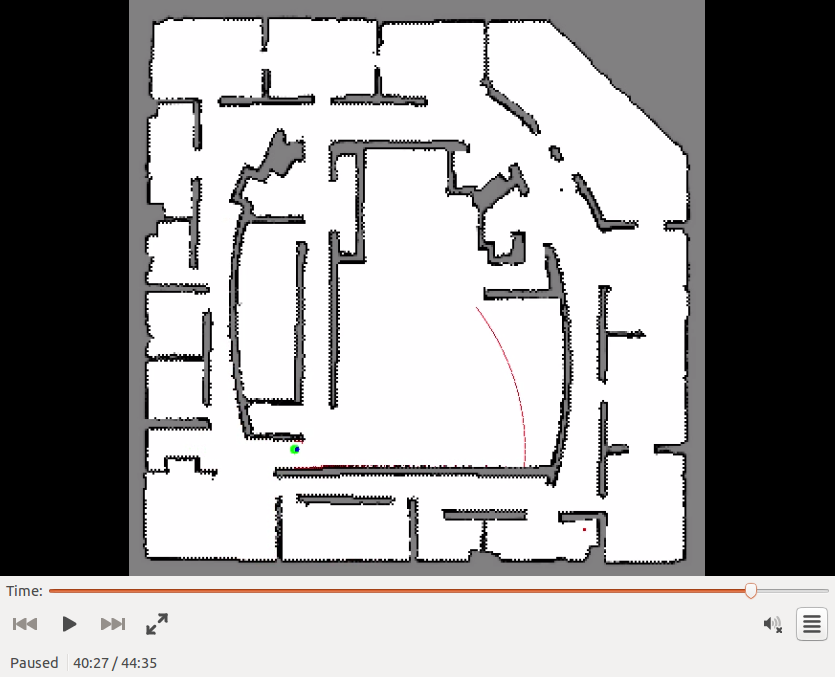
\includegraphics[trim = {4.6cm 3.8cm 4.6cm 0}, clip, width=\textwidth]{40min.png}
%%        \caption*{$t=40$ min}
%%        \label{fig:IRL40min}
%%    \end{subfigure}
%    \caption*{A robot (green) measures a room in ROS Stage simulator using modified Intel Research Lab floor plan using the proposed mapping and exploration algorithms.}
%    \label{fig:IRL}
%\end{figure}
%
%
%\end{frame}
%
%
%
%
%
%\begin{frame}
%\frametitle{Experimental Example}
%\begin{itemize}
%        	\item A pioneer ground vehicle explores a room composed of Styrofoam walls
%	\item Experiments use ROS, a Microsoft Kinect depth sensor, and Vicon Tracker for pose information
%\end{itemize}
%\begin{figure}
%	\centering
%    	\begin{subfigure}[b]{0.28\textwidth}
%        		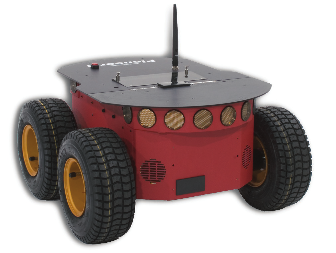
\includegraphics[width=\textwidth]{pioneer.png}
%        		\caption*{Pioneer}
%    	\end{subfigure}    	
%	\hspace*{0.04\textwidth}
%	\begin{subfigure}[b]{0.28\textwidth}
%        		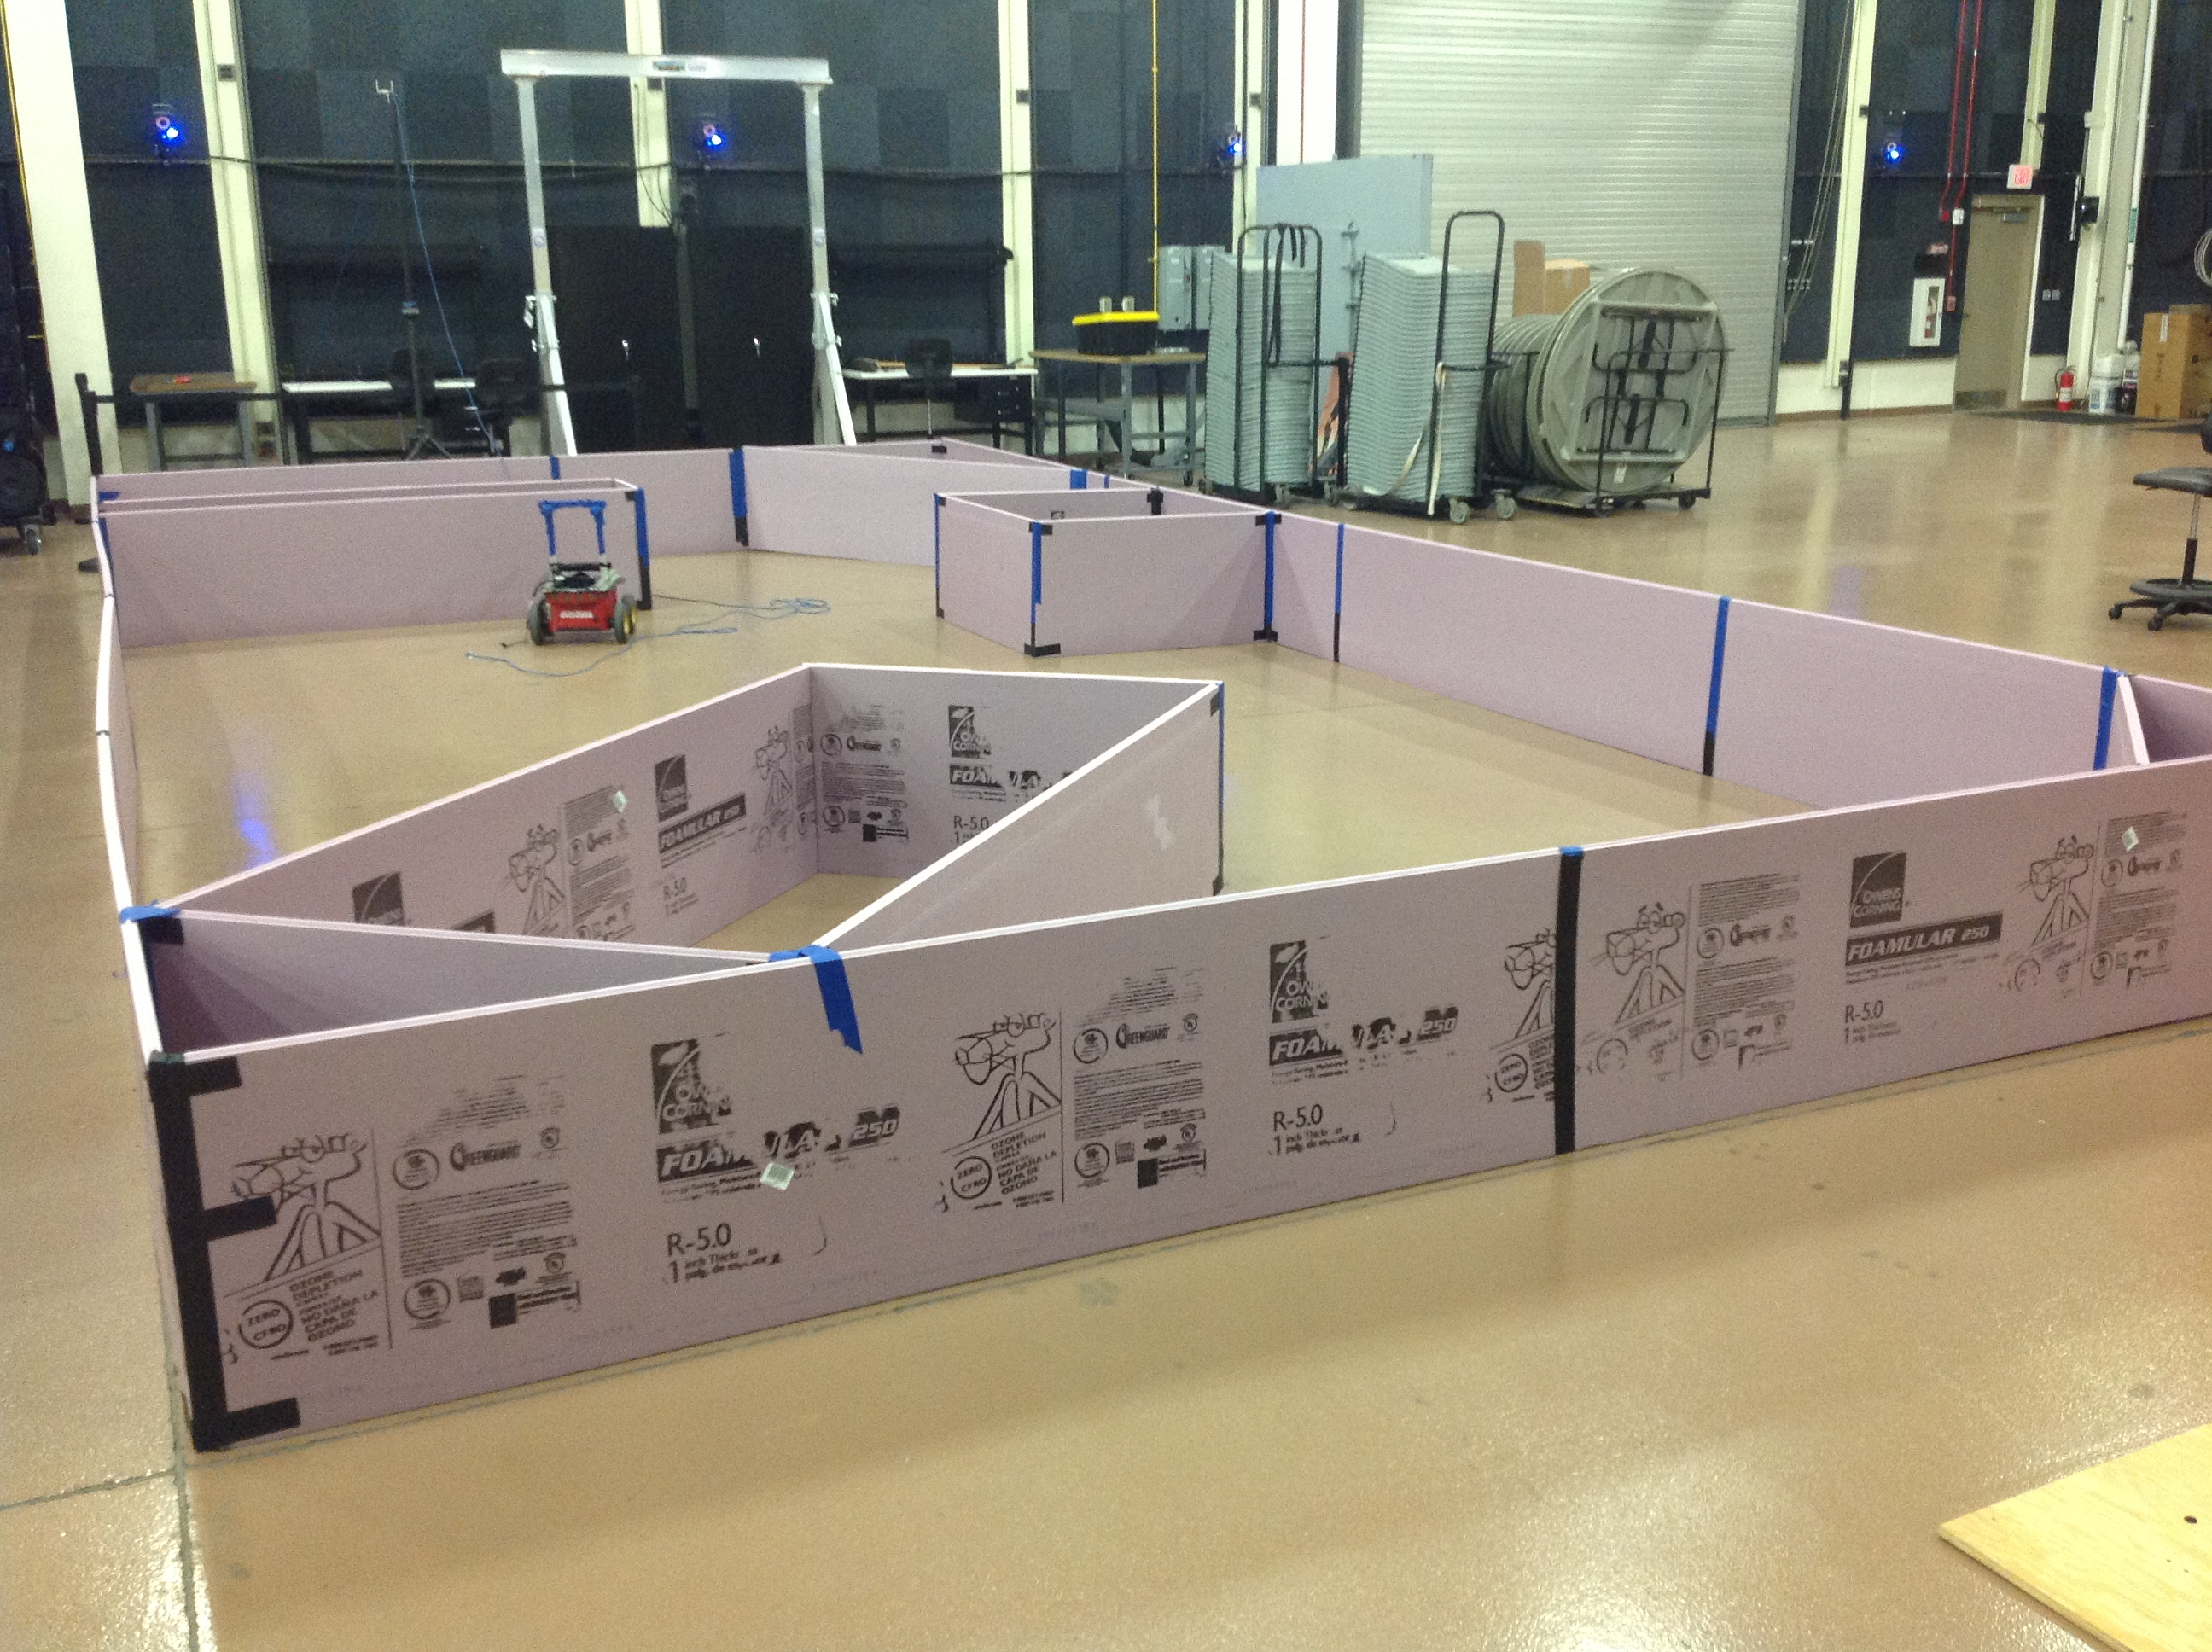
\includegraphics[width=\textwidth]{test_setup_1.jpg}
%        		\caption*{Bottom-left view}
%    	\end{subfigure}
%	\hspace*{0.03\textwidth}
%	\begin{subfigure}[b]{0.28\textwidth}
%        		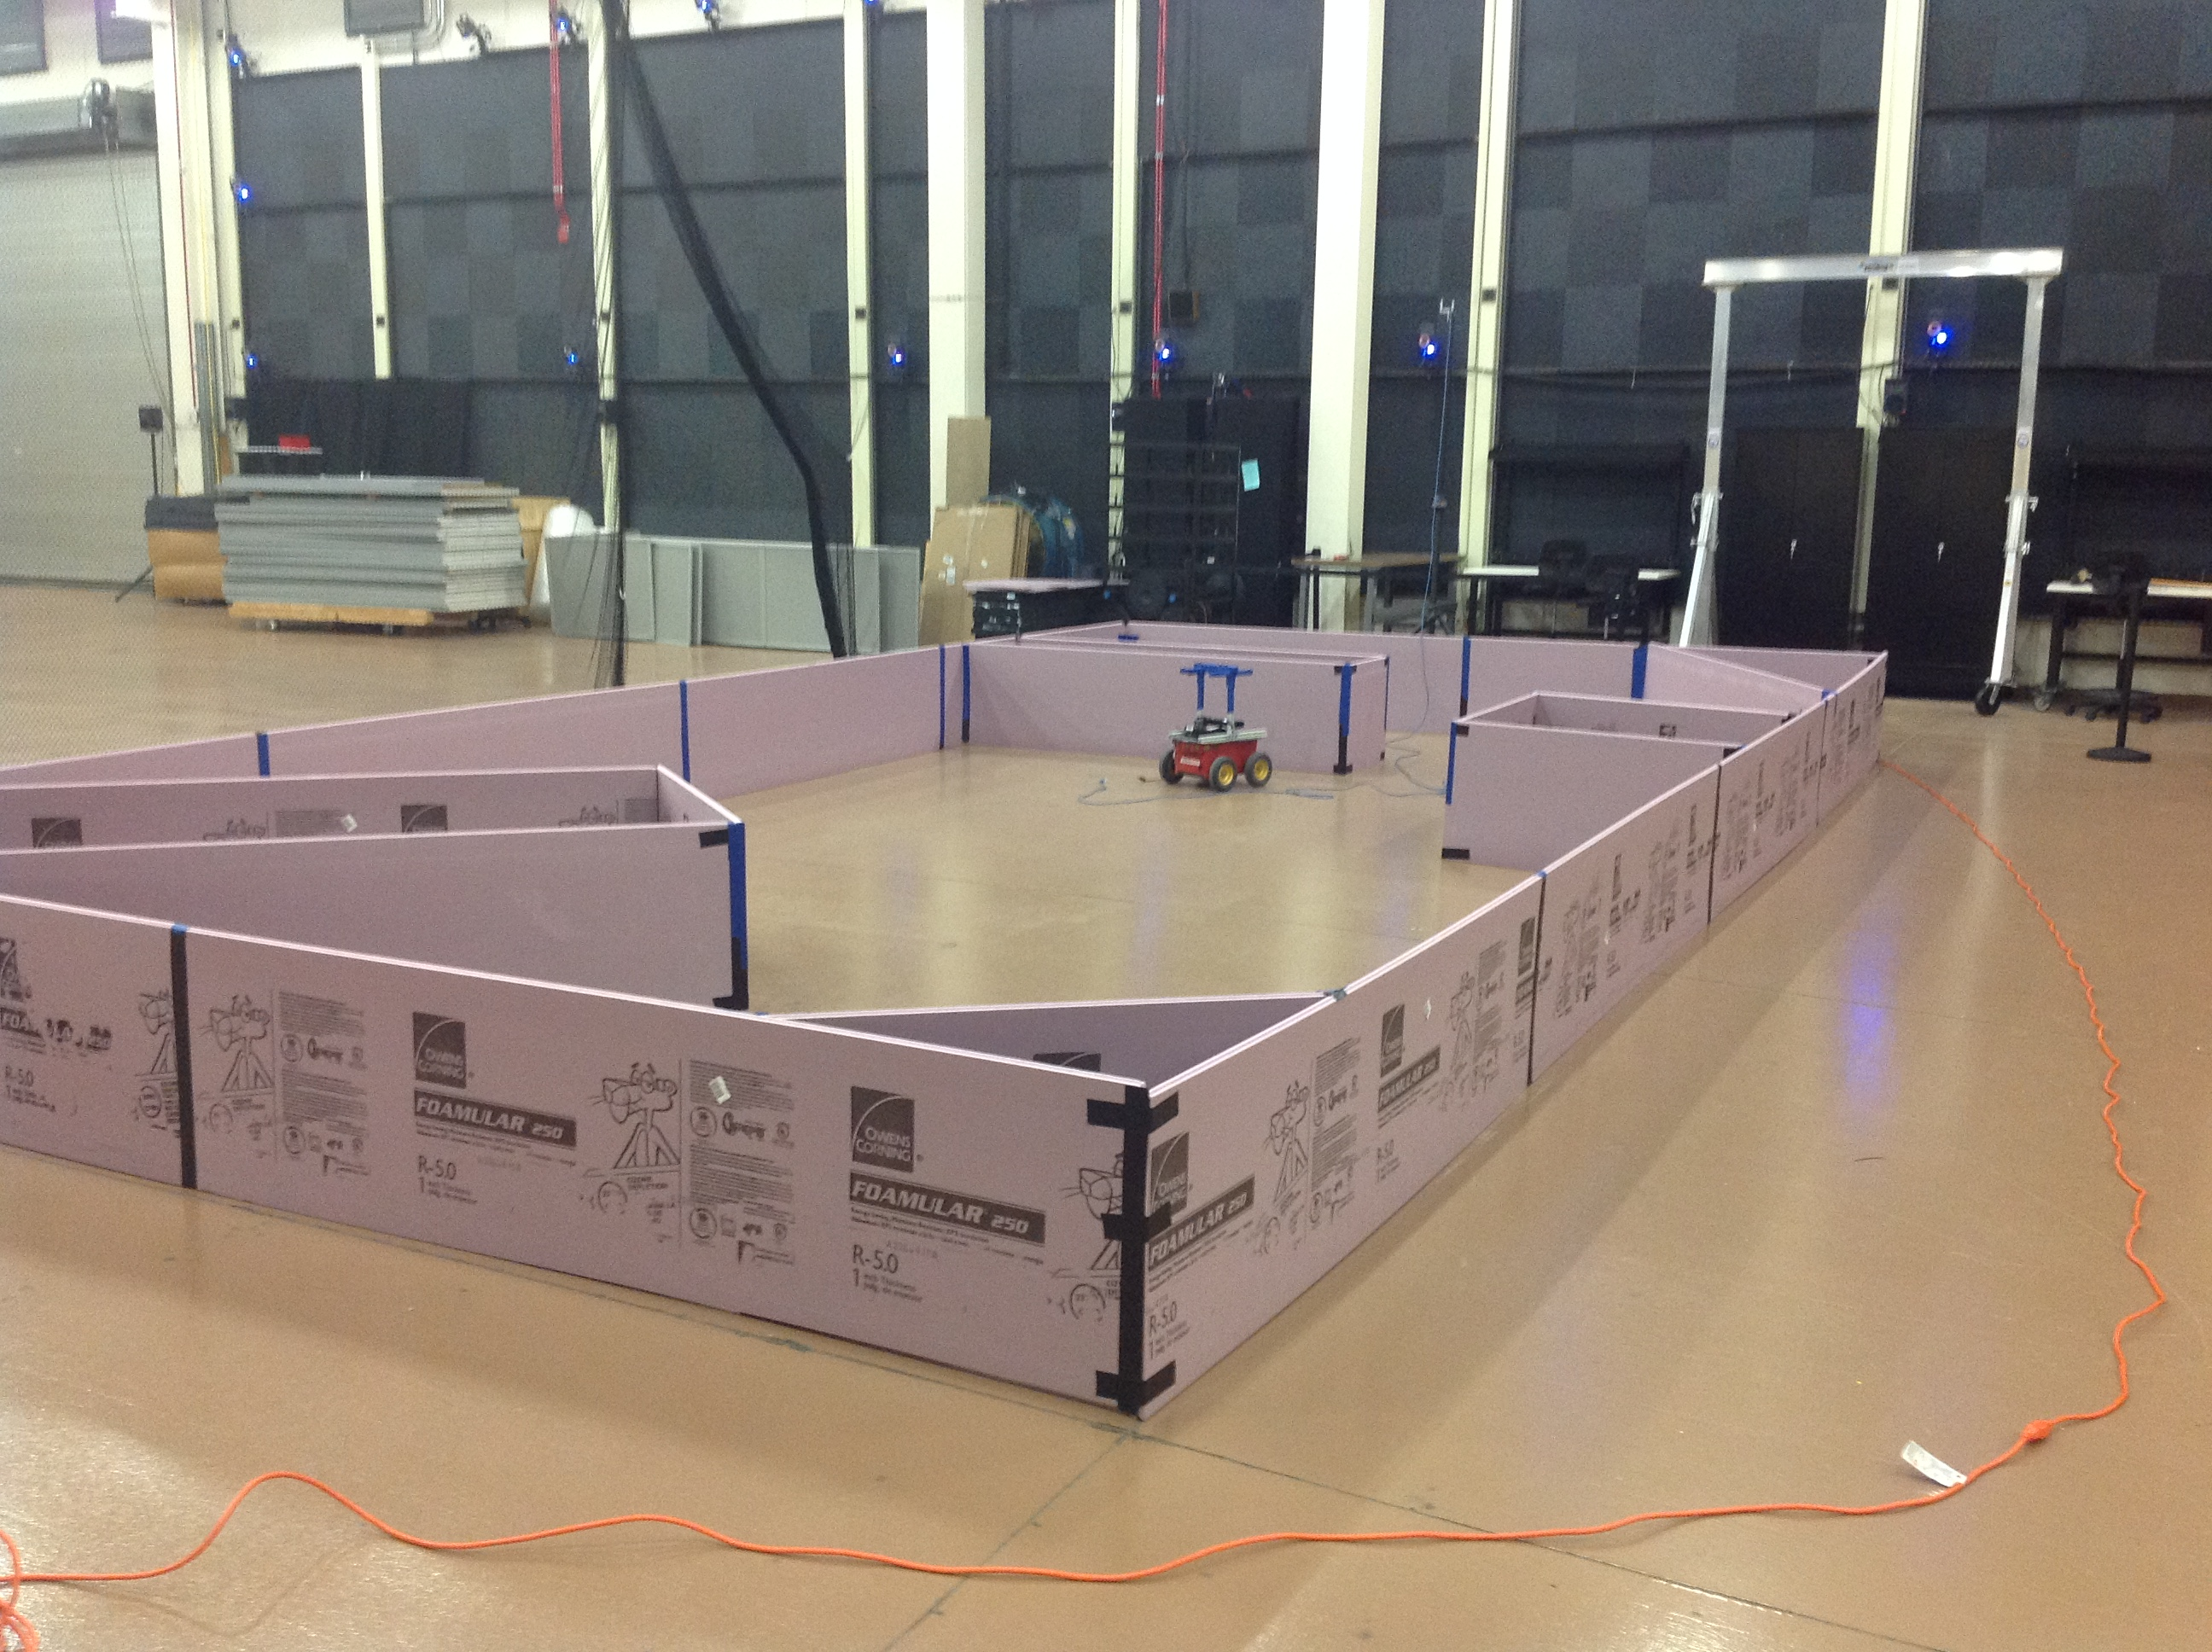
\includegraphics[width=\textwidth]{test_setup_2.jpg}
%        		\caption*{Bottom-right view}
%    	\end{subfigure}
%\end{figure}
%
%\end{frame}
%
%%\begin{frame}
%%\frametitle{Experimental Results}
%%	\centering{
%%	\includemovie[poster,autoplay]{0.720\textwidth}{0.576\textwidth}{../../Fig/JIRS16_experiment_SideBySide_speedup8x.mov}}
%%\end{frame}
%
%\begin{frame}
%\frametitle{Experimental Results}
%
%\begin{figure}
%	\centering{
%    	\begin{subfigure}[b]{0.19\textwidth}
%        		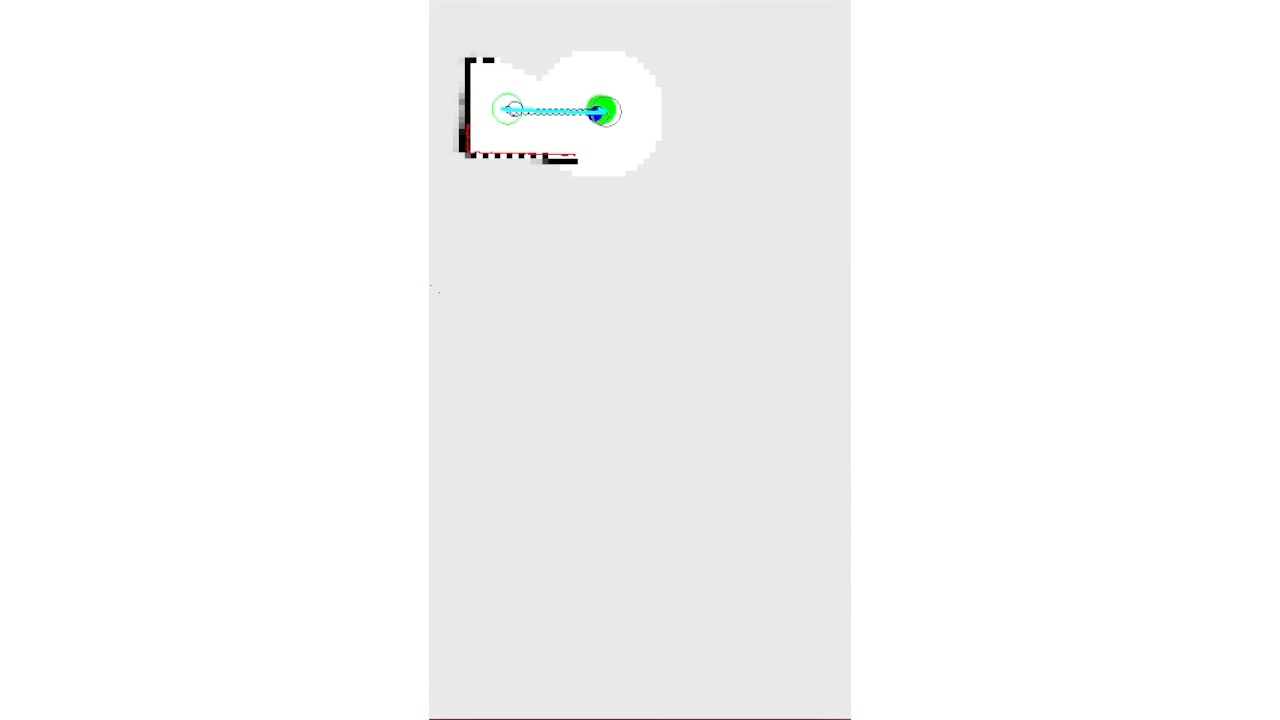
\includegraphics[trim={13cm 1cm 13cm 0}, clip, width=\textwidth]{t_start.jpg}
%        		\caption*{$t=0.0$min}
%        		\label{fig:Experiment_ogm_t0}
%    	\end{subfigure}
%	\begin{subfigure}[b]{0.19\textwidth}
%        		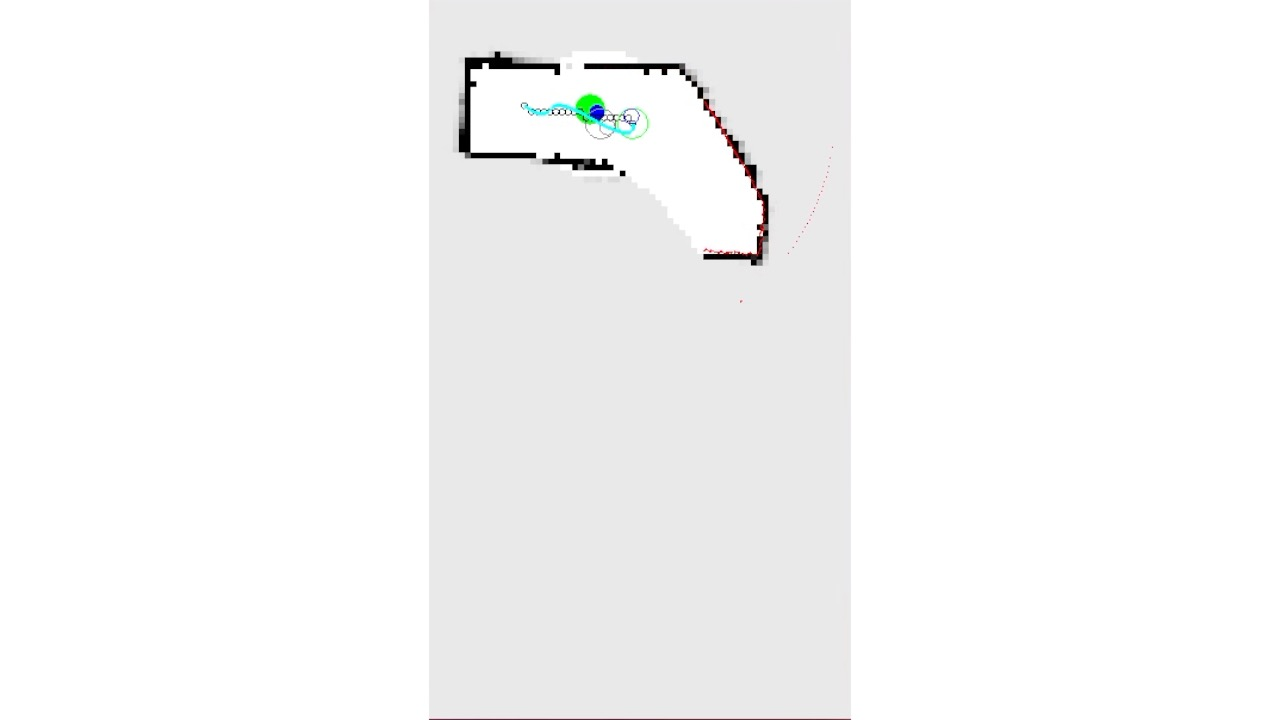
\includegraphics[trim={13cm 1cm 13cm 0}, clip, width=\textwidth]{t_0p5min.jpg}
%        		\caption*{$t=0.5$min}
%        		\label{fig:Experiment_ogm_t0p5}
%    	\end{subfigure}    
%	\begin{subfigure}[b]{0.19\textwidth}
%        		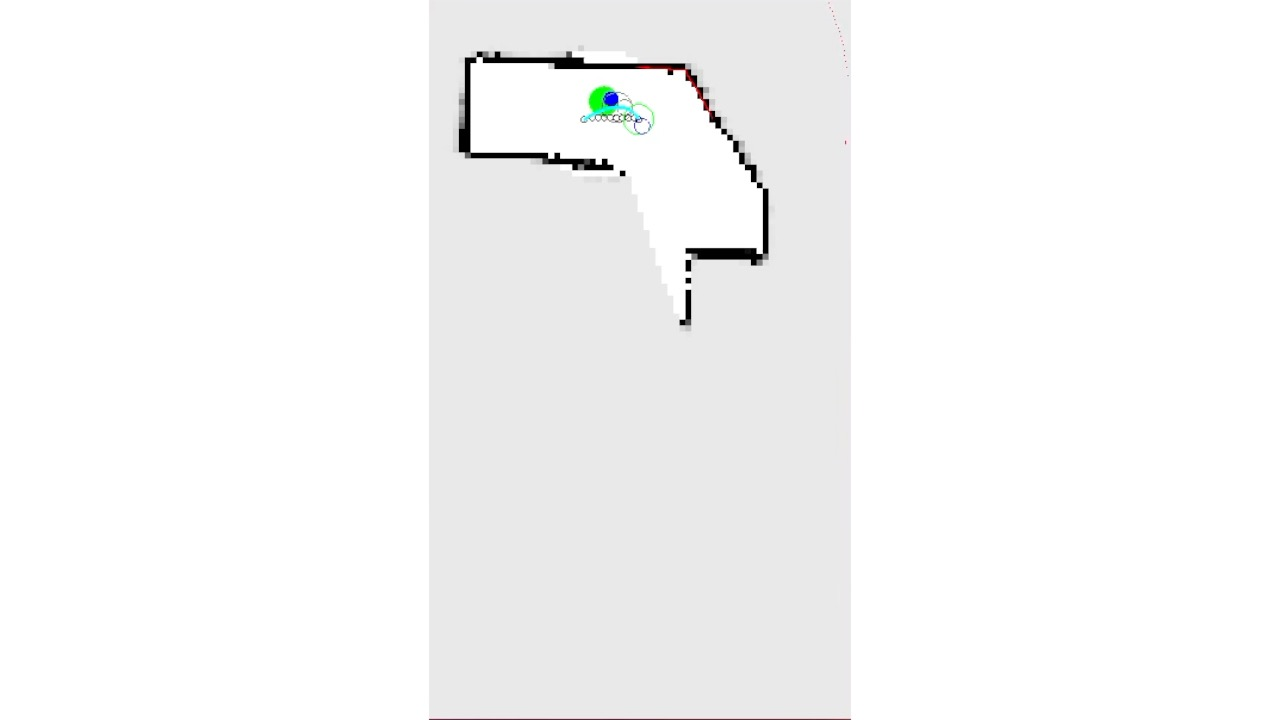
\includegraphics[trim={13cm 1cm 13cm 0}, clip, width=\textwidth]{t_1min.jpg}
%        		\caption*{$t=1.0$min}
%        		\label{fig:Experiment_ogm_t1}
%    	\end{subfigure}
%	\begin{subfigure}[b]{0.19\textwidth}
%        		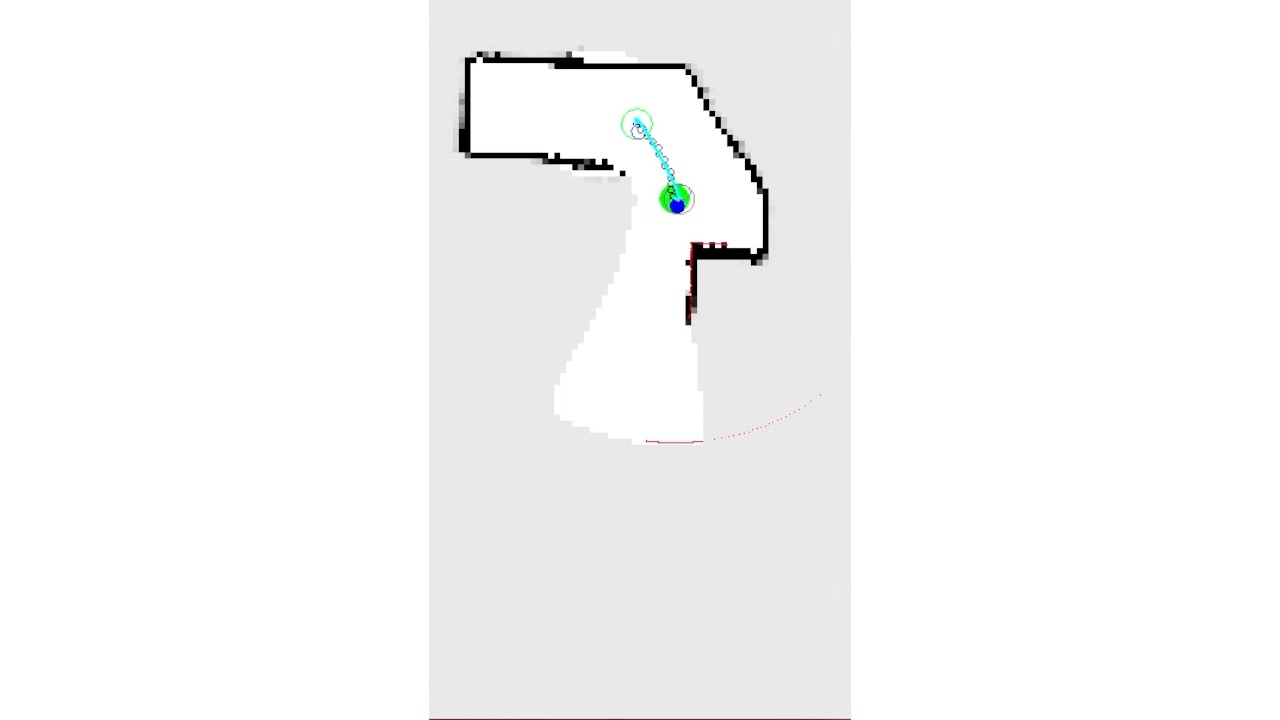
\includegraphics[trim={13cm 1cm 13cm 0}, clip, width=\textwidth]{t_1p5min.jpg}
%        		\caption*{$t=1.5$min}
%        		\label{fig:Experiment_ogm_t1p5}
%    	\end{subfigure}
%	\begin{subfigure}[b]{0.19\textwidth}
%        		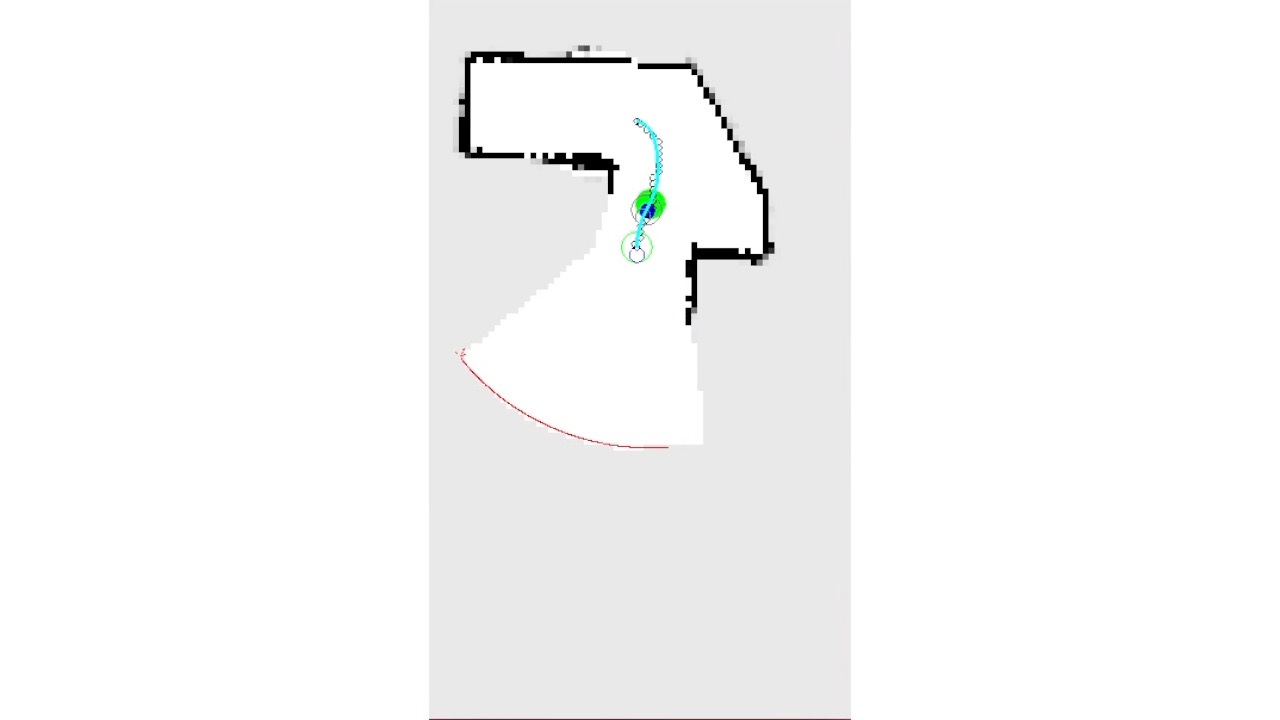
\includegraphics[trim={13cm 1cm 13cm 0}, clip, width=\textwidth]{t_2min.jpg}
%        		\caption*{$t=2.0$min}
%        		\label{fig:Experiment_ogm_t2}
%    	\end{subfigure}
%		\vspace*{0.05\textwidth}
%
%	}
%	\vspace*{-1cm}
%	\centering{
%    	\begin{subfigure}[b]{0.19\textwidth}
%        		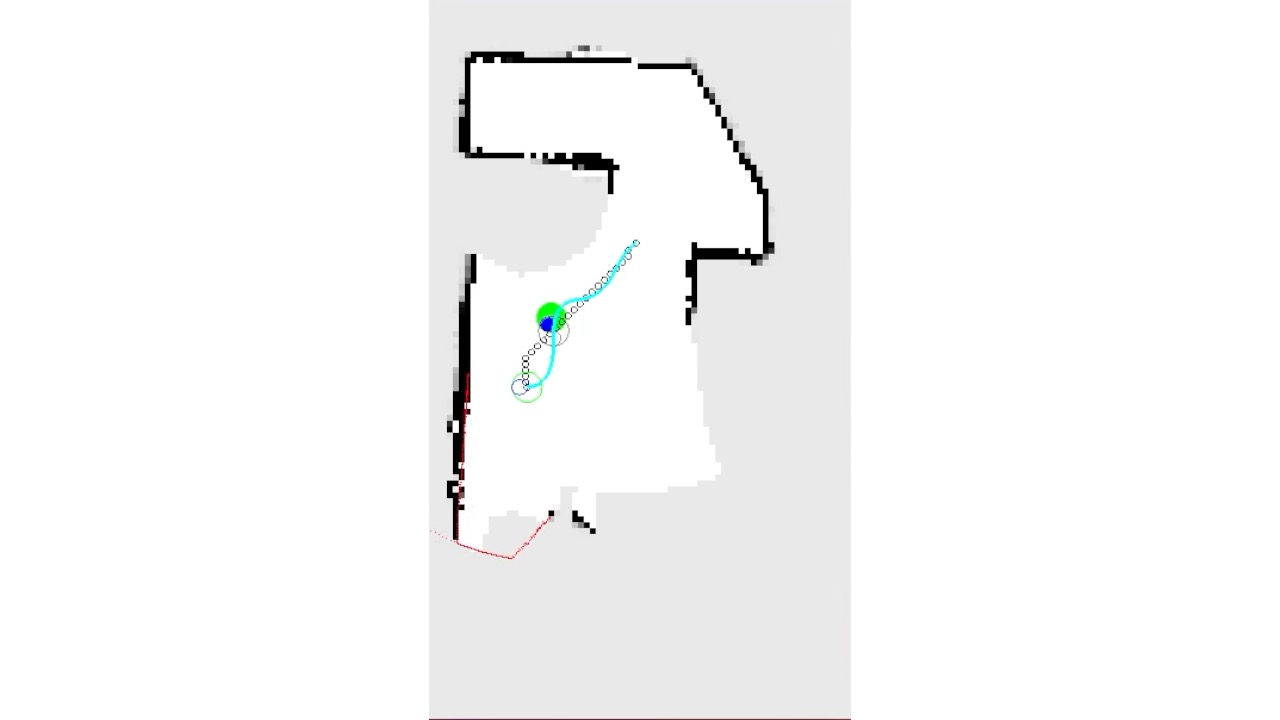
\includegraphics[trim={13cm 1cm 13cm 0}, clip, width=\textwidth]{t_2p5min.jpg}
%        		\caption*{$t=2.5$min}
%        		\label{fig:Experiment_ogm_t2p5}
%    	\end{subfigure}
%	\begin{subfigure}[b]{0.19\textwidth}
%        		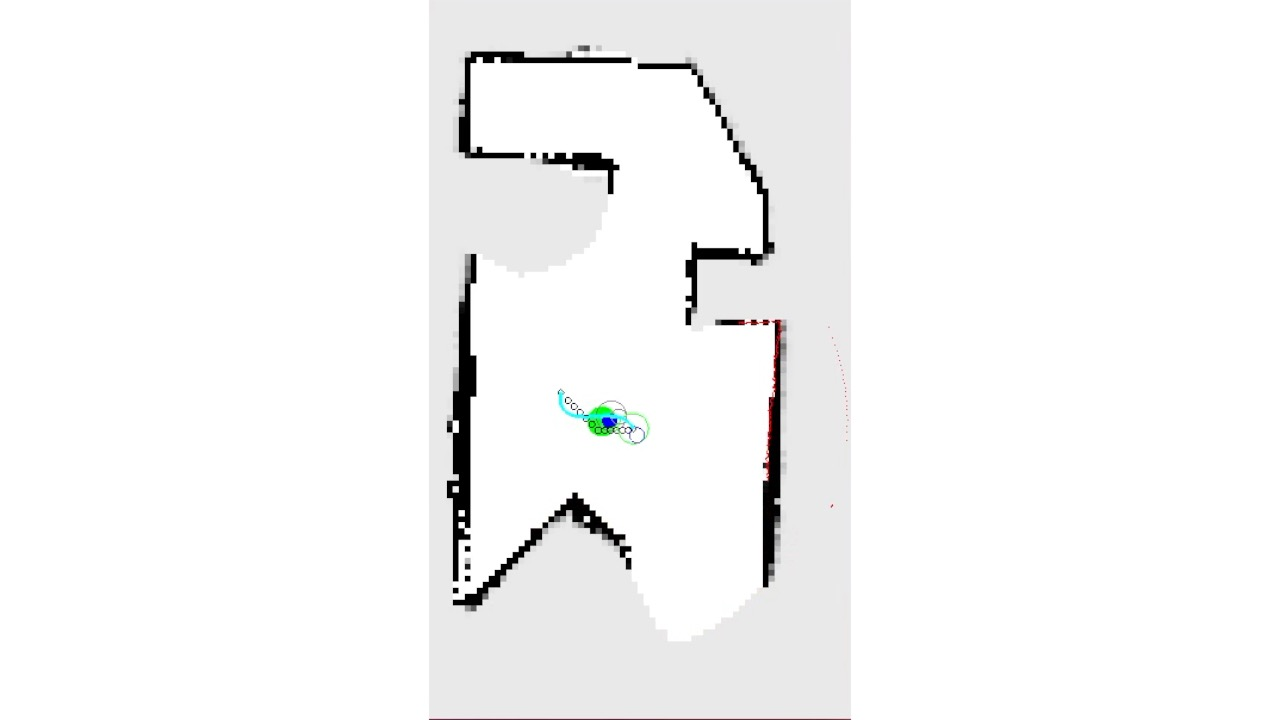
\includegraphics[trim={13cm 1cm 13cm 0}, clip, width=\textwidth]{t_3min.jpg}
%        		\caption*{$t=3.0$min}
%        		\label{fig:Experiment_ogm_t3}
%    	\end{subfigure}    
%	\begin{subfigure}[b]{0.19\textwidth}
%        		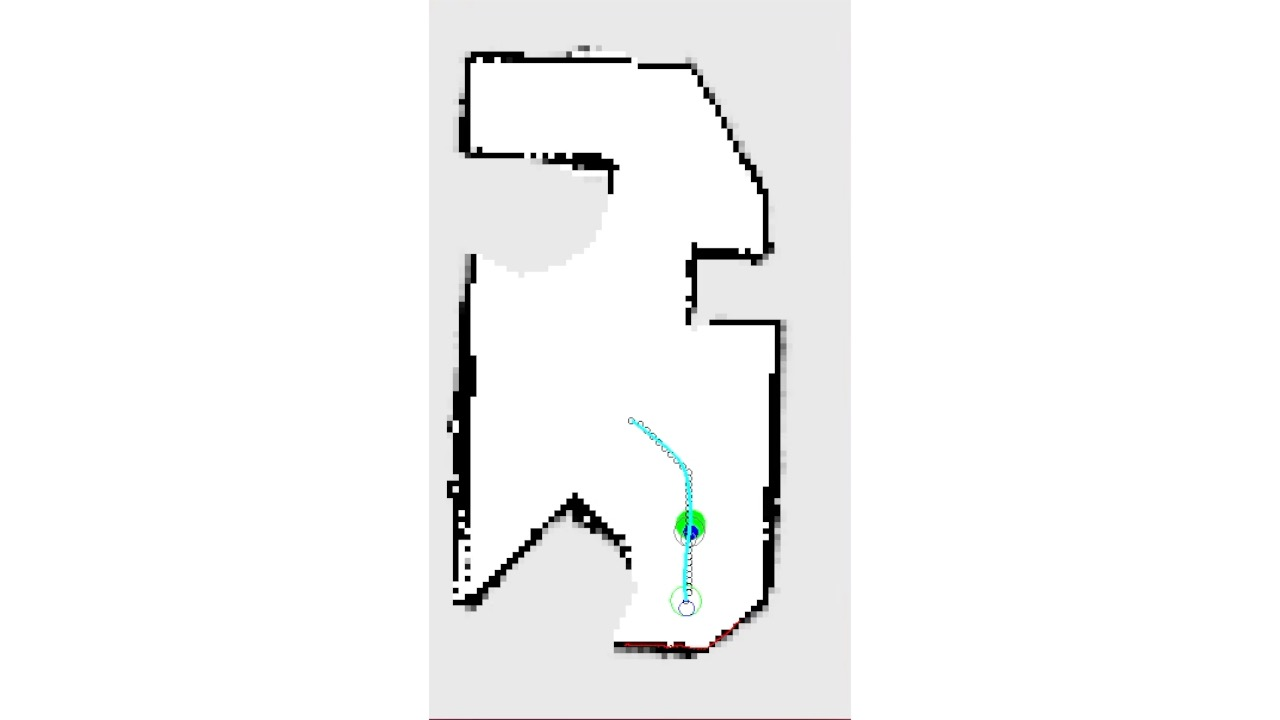
\includegraphics[trim={13cm 1cm 13cm 0}, clip, width=\textwidth]{t_3p5min.jpg}
%        		\caption*{$t=3.5$min}
%        		\label{fig:Experiment_ogm_t3p5}
%    	\end{subfigure}
%	\begin{subfigure}[b]{0.19\textwidth}
%        		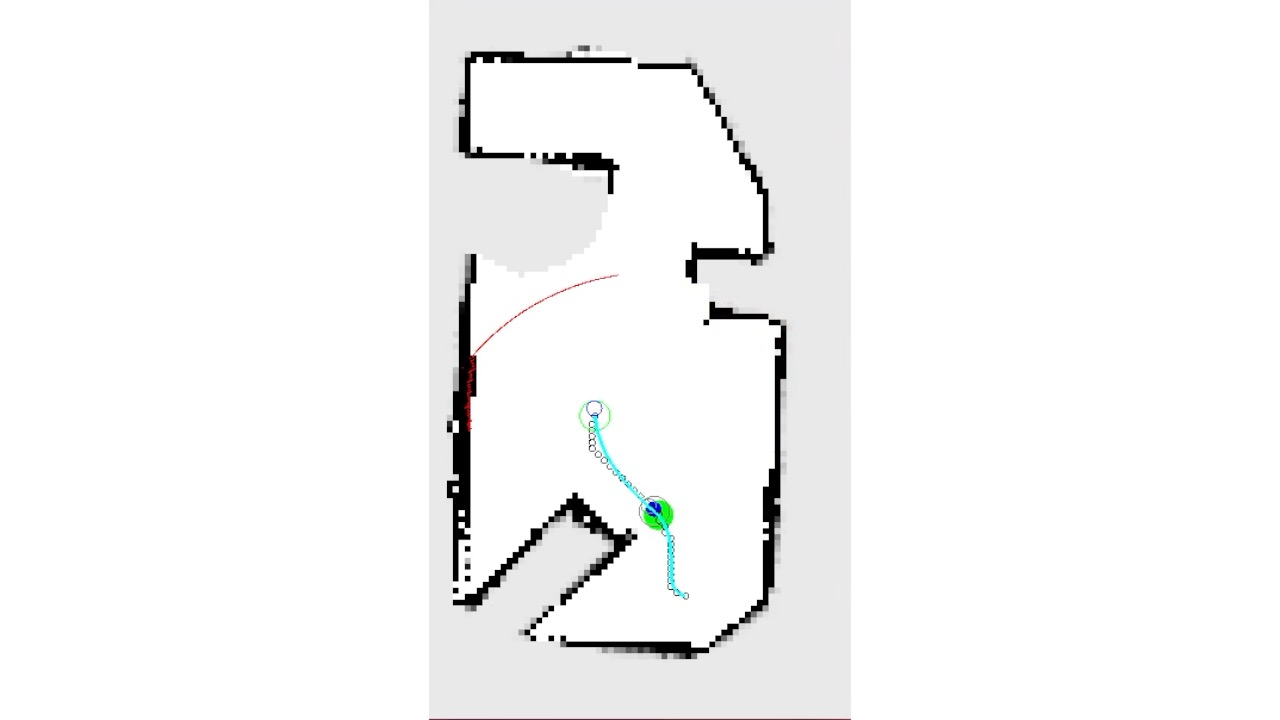
\includegraphics[trim={13cm 1cm 13cm 0}, clip, width=\textwidth]{t_4min.jpg}
%        		\caption*{$t=4.0$min}
%        		\label{fig:Experiment_ogm_t4}
%    	\end{subfigure}
%	\begin{subfigure}[b]{0.19\textwidth}
%        		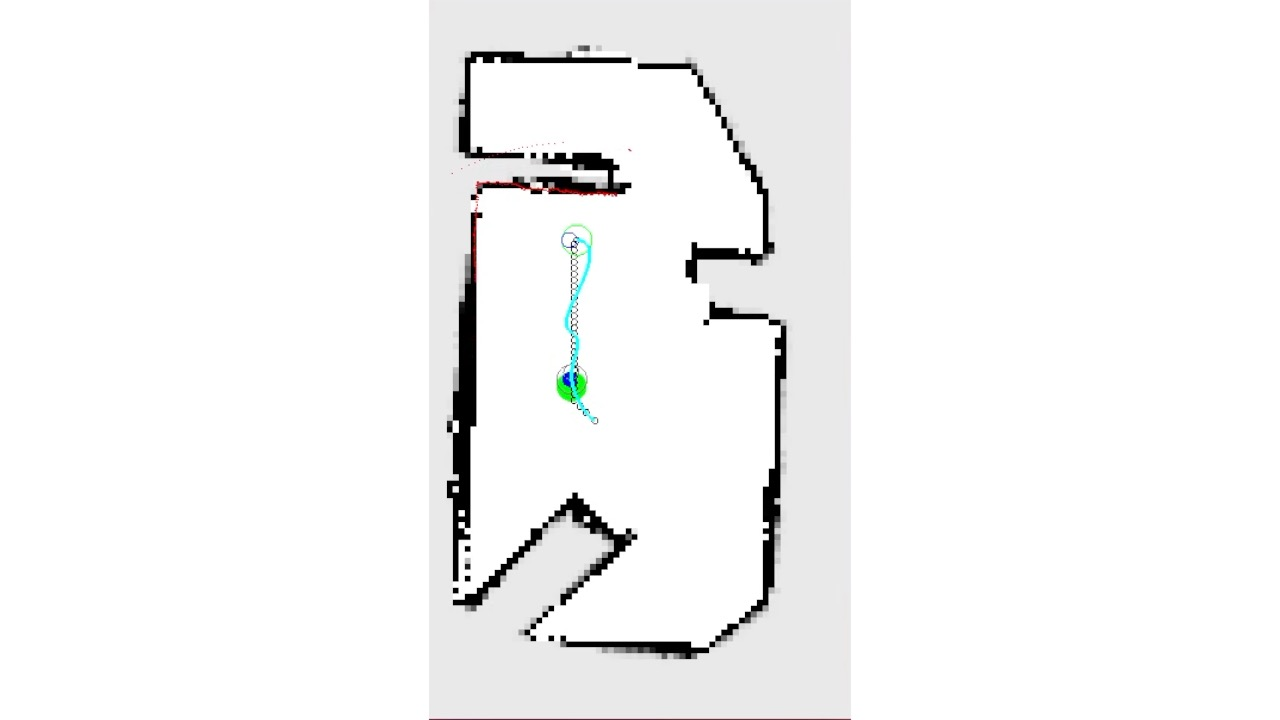
\includegraphics[trim={13cm 1cm 13cm 0}, clip, width=\textwidth]{t_4p5min.jpg}
%        		\caption*{$t=4.5$min}
%        		\label{fig:Experiment_ogm_t4p5}
%    	\end{subfigure}
%	}
%\end{figure}
%
%\end{frame}
%
%
%
%\section*{}
%
%\begin{frame}
%\frametitle{}
%%\center
%\center{\bf \color{blue} Future Direction:\\Multi-Robot Autonomous Exploration}
%\end{frame}
%
%\subsection*{Future Direction: Multi-Robot Autonomous Exploration}
%
%\begin{frame}
%\frametitle{Proposed Topics}
%\begin{itemize}
%        	\item The ray-by-ray exact occupancy grid mapping approach in centralized probabilistic mapping
%	\item Multiple robots choosing optimal motions considering each other
%	\item Robots avoiding collisions with each other
%	\item Coverage optimization of robots from different poses
%\end{itemize}
%
%\end{frame}
%
%\begin{frame}
%\frametitle{Proposed Future Steps}
%\begin{itemize}
%        	\item Mapping:
%	\begin{itemize}
%		\item Restructure algorithms for centralized map generation
%		\item Communicate with multiple measurement sources
%	\end{itemize}
%	\item Exploration:
%	\begin{itemize}
%		\item Simplify enormous computation: bidding-based approach
%		\item Temporary theoretical map building
%		\item Collision avoidance between robots
%	\end{itemize}
%\end{itemize}
%
%\end{frame}
%
%
%
%\section*{}
%
%\begin{frame}
%\frametitle{}
%%\center
%\center{\bf \color{blue} Conclusions and Publications}
%\end{frame}
%
%
%\subsection*{Conclusions and Publications}
%
%\begin{frame}
%\frametitle{Conclusions}
%\begin{itemize}
%        	\item Proposed an occupancy grid mapping technique that uses the \emph{exact probabilistic solution}
%	\item Computational cost is reduced \emph{substantially} for \emph{real-time implementation} using probabilisitic properties and exploiting mathematical patterns
%	\item Exact mapping concepts are extended to map uncertainty to accomplish \emph{autonomous exploration}
%	\item Proposing multiple vehicles can explore an uncertain environment using a \emph{bidding}-based approach
%\end{itemize}
%\end{frame}

% TODO: update with dissertation version!

\begin{frame}
\frametitle{Publications on Dissertation Topics}
{\tiny 
\begin{itemize}
	\item E. Kaufman, K. Takami, T. Lee, and Z. Ai, ``Multi-Vehicle Cooperative Exploration and Patrol of Uncertain 3D Environments'', in preparation.
	\item E. Kaufman, K. Takami, T. Lee, and Z. Ai, ``Bidding-Based Autonomous Exploration of Cooperative Robots Building a 3D Probabilistic Occupancy Grid Map'', in preparation.
	\item E. Kaufman and T. Lee, ``Autonomous Aerial Exploration for Topological Mapping of Mars Environments'', \textit{2019 AIAA Guidance, Navigation, and Control Conference}, San Diego, CA, January 2019, submitted.
	\item E. Kaufman, K. Takami, Z. Ai, and T. Lee, ``Autonomous Quadrotor 3D Mapping and Exploration Using Exact Occupancy Probabilities,'' \textit{The Second IEEE International Conference on Robotic Computing}, pp. 49--55, Laguna Hills, CA, January 2018.
	\item E. Kaufman, K. Takami, T. Lee, and Z. Ai, ``Autonomous Exploration with Exact Inverse Sensor Models,'' \textit{Journal of Intelligent }\&\textit{ Robotic Systems}, 2017, doi: 10.1007/s10846-017-0710-7.
	\item E. Kaufman, T. Lee, and Z. Ai, ``Autonomous Exploration by Expected Information Gain from Probabilistic Occupancy Grid Mapping,'' \textit{IEEE International Conference on Simulation, Modeling, and Programming for Autonomous Robots}, pp. 246--251, San Francisco, CA, December 2016.
	\item E. Kaufman, T. Lee, Z. Ai, and I. S. Moskowitz, ``Bayesian Occupancy Grid Mapping via an Exact Inverse Sensor Model,'' \textit{Proceedings of the American Control Conference}, pp. 5709-5715, Boston, MA, July 2016.
\end{itemize}
}
\end{frame}

\begin{frame}
\frametitle{Publications on Data Association, Estimation, and Control}
{\tiny 
\begin{itemize}
	\item E. Kaufman, T. A. Lovell, and T. Lee, ``Nonlinear Observability Measure for Relative Orbit Determination with Angles-Only Measurements,'' \textit{The Journal of the Astronautical Sciences}, 63(1): pp. 60-80, 2016, doi: 10.1007/s40295-015-0082-9.
	\item E. Kaufman, T. A. Lovell, and T. Lee, ``Minimum Uncertainty JPDA Filters and Coalescence Avoidance for Multiple Object Tracking,'' \textit{The Journal of the Astronautical Sciences}, 63(4): pp. 308-334, 2016, doi: 10.1007/s40295-016-0092-2.
	\item T. Wu, E. Kaufman, and T. Lee, ``Globally Asymptotically Stable Attitude Observer on SO(3),'' \textit{Proceedings of the 54th IEEE Conference on Decision and Control}, pp. 2164-2168, Osaka, Japan, December 2015.
	\item E. Kaufman, T. A. Lovell, and T. Lee, ``Nonlinear Observability Measure for Relative Orbit Determination with Angles-Only Measurements,'' \textit{Proceedings of the 25th AAS/AIAA Space Flight Mechanics Meeting}, AAS 15-451, Williamsburg, VA, January 2015.
	\item E. Kaufman, T. A. Lovell, and T. Lee, ``Minimum Uncertainty JPDA Filter and Coalescence Avoidance Performance Evaluations,'' \textit{Proceedings of the 25th AAS/AIAA Space Flight Mechanics Meeting, Williamsburg}, AAS 15-432, VA, January 2015.
	\item E. Kaufman, K. Caldwell, D. Lee, and T. Lee, ``Design and Development of a Free-Floating Hexrotor UAV for 6-DOF Maneuvers,'' \textit{Proceedings of the IEEE Aerospace Conference}, ASC 14-2527, March 2014, Big Sky, MT.
	\item E. Kaufman, T. A. Lovell, and T. Lee, ``Optimal Joint Probabilistic Data Association Filter Avoiding Coalescence in Close Proximity,'' \textit{Proceedings of the European Control Conference}, pp. 2709-2714, Strasbourg, June 2014.
\end{itemize}
}
\end{frame}




\end{document}

